\chapter{Desenvolvimento \label{CAP:DESENVOLVIMENTO}}
\vspace{-2.5 cm}

% Este Capítulo apresenta o que foi desenvolvido até o momento.
Este Capítulo apresenta o que foi desenvolvido como resultado deste trabalho,
visando alcançar os objetivos propostos.

\section{Desenvolvimento dos controladores}

	Nesta seção pretende-se investigar a arquitetura comportamental em robótica 
	móvel para as duas estratégias clássicas de implementação: arbitragem e fusão de 
	comportamentos. Para isso, controladores híbrido e fuzzy serão criados, o primeiro
	para arbitragem e o segundo para fusão.

	\subsection{Controle de sistema híbrido}
	
	Nesta subseção, pretende-se demonstrar um controlador simples capaz de 
	solucionar o problema de navegação, usando autômato híbrido. Para cada estado
	no autômato, um controlador é selecionado e uma recomendação de saída é 
	calculada. 
	
	A recomendação para todos os comportamentos é dada por um vetor. Seu ângulo é calculado 
	para  o sistema de coordenadas global e, subtraindo o ângulo do robô, o erro é calculado. 
	A partir do erro, um controlador PID calcula a velocidade angular. 
		
	O cálculo efetuado pelo controlador PID é mostrado na Equação \ref{eq:controladorPID},
	onde $\omega$ é a velocidade angular, $\epsilon(k)$ é o erro para a k-ésima iteração e 
	$T$ é o período de amostragem.
	\begin{equation}
		\label{eq:controladorPID}
		\omega = K_p \epsilon(k) + K_i \sum_0^k \epsilon(k) T + k_d \frac{\epsilon(k) - \epsilon(k-1)}{T}
	\end{equation}
	
	A saída do controlador PID fornece uma recomendação para velocidade angular do modelo uniciclo. 
	A velocidade linear é arbitrária e inicialmente é definida como a velocidade máxima 
	do robô, mas cada comportamento tem a prerrogativa de alterá-la, caso necessário.
	
	A Equação \ref{eq:vw_to_diff}, se utilizada diretamente, pode retornar valores de 
	$w_l$ e $w_r$ saturados ou em região de zona morta. Pode-se concluir que a velocidade linear 
	é uma recomendação de baixa prioridade em relação à velocidade angular, já que só é possível 
	seguir ângulo definindo essa prioridade.
	
	É necessário utilizar um algoritmo para reduzir velocidade linear caso recomendação ultrapasse 
	limites máximos, a fim de atender recomendação de velocidade angular. O Algoritmo 
	\ref{alg:ensurew} mostra o procedimento capaz de garantir a conversão segura entre modelo
	uniciclo e de acionamento diferencial. 
		
	\begin{algorithm}
	\caption{Uniciclo para Acionamento Diferencial priorizando $\omega$}
	\label{alg:ensurew}%
	\begin{algorithmic}[1]
	
	\REQUIRE $v, \omega$
	\ENSURE $\omega_l, \omega_r$
	
	\IF{$v > 0$}
		\STATE $vlim \leftarrow max(min(abs(v), R \cdot VEL\_MAX), R \cdot VEL\_MIN)$
		\STATE $wlim \leftarrow max(min(abs(\omega), (R/L) \cdot (VEL\_MAX - VEL\_MIN)), 0)$
		
		\STATE $w_{l,lim}, w_{r,lim} \leftarrow uniToDiff(vlim, wlim)$
		
		\STATE $ velocidadeMaior \leftarrow max(w_{l,lim}, w_{r,lim})$
		\STATE $ velocidadeMenor \leftarrow min(w_{l,lim}, w_{r,lim})$
	
		\IF{$velocidadeMaior > VEL\_MAX$}
			\STATE $w_{l,lim} \leftarrow w_{l,lim} - (velocidadeMaior - VEL\_MAX)$
			\STATE $w_{r,lim} \leftarrow w_{r,lim} - (velocidadeMaior - VEL\_MAX)$
		\ELSIF{$velocidadeMenor < VEL\_MIN$}
			\STATE $w_{l,lim} \leftarrow w_{l,lim} + (VEL\_MIN - velocidadeMenor)$
			\STATE $w_{r,lim} \leftarrow w_{r,lim} + (VEL\_MIN - velocidadeMenor)$
		\ENDIF
		
		\IF{$v \geq 0$}
			\STATE $vlim \leftarrow 1$
		\ELSE
			\STATE $vlim \leftarrow -1$
		\ENDIF
			
		\IF{$\omega \geq 0$}
			\STATE $wlim \leftarrow 1$
		\ELSE
			\STATE $wlim \leftarrow -1$
		\ENDIF
			
		\STATE $v,\omega \leftarrow diffToUni(w_{l,lim},w_{r,lim})$
		\STATE $v \leftarrow v \cdot vlim$
		\STATE $\omega \leftarrow \omega \cdot wlim$
	\ELSE
		\IF{$abs(\omega) > (R/L) \cdot 2 \cdot VEL\_MIN$}
			\IF{$\omega \geq 0$}
				\STATE $\omega \leftarrow max(min(abs(\omega),(R/L) \cdot 2 \cdot VEL\_MAX),(R/L) \cdot 2 \cdot VEL\_MIN)$ 
			\ELSE
				\STATE $\omega \leftarrow -max(min(abs(\omega),(R/L) \cdot 2 \cdot VEL\_MAX),(R/L) \cdot 2 \cdot VEL\_MIN)$
			\ENDIF
		\ELSE
			\STATE $\omega \leftarrow 0$
		\ENDIF
	\ENDIF
		
	\STATE $\omega_l, \omega_r \leftarrow uniToDiff(v,\omega)$
	
	\end{algorithmic}
	\end{algorithm}

	A ideia desse algoritmo é verificar se há saturação e, caso positivo, a diferença entre
	velocidade sugerida e velocidade máxima permitida pelos motores é subtraída de $w_l$ e 
	$w_r$. Além de respeitar o limite superior de velocidade, o limite inferior (região de 
	zona morta) também é respeitado e, se necessário, a diferença é somada para garantir que
	não há travamento de motores devido a atrito.
		
	As funções ``uniToDiff()'' e ``diffToUni()'' efetuam as conversões de modelos matemáticos
	das Equações \ref{eq:vw_to_diff} e \ref{eq:diff_to_vw}, respectivamente.
	
		\subsubsection{Comportamento ``Ir Para Objetivo'' \label{SEC:IPO}}
		
		O comportamento ``Ir Para Objetivo'', exemplificado na Figura \ref{fig:CompIPO}, calcula 
		um vetor objetivo a partir do centro de massa do robô. A Equação 
		\ref{eq:vetor_ipo_calculo} mostra o cálculo, onde $P_o$ e $P_r$ são pontos que podem ser 
		vistos na Figura. A recomendação para velocidade linear é a máxima, já que o robô 
		está livre de obstáculos.
		
		\newcommand{\meuRoboLindaoCompIPO}{
	\begin{tikzpicture}[scale = 2]%
		\coordsystwo{I}
		\begin{scope}[shift={(3, 0.9)}]
			\draw[->] (0.3,0) arc (0:30:0.3);
			\draw[-] (0,0) -- (0.4,0);
			\node at (0.5,0.1) {$\phi$};
			
			% Pr 
			\begin{scope}[scale = 0.5]
				\node[color = gray] at (0.1,-0.35) {$P_r$};
			\end{scope}
			\begin{scope}[rotate=30,scale=0.5]
				\begin{scope}[scale=0.9]
					\coordsystwo{R}
				\end{scope}
				\begin{scope}[shift={(0.25,0)},rotate = -90]
					\RoboDiffClean
				\end{scope}
			\end{scope}	
		\end{scope}
		
		% Coord objetivo
		\begin{scope}[shift={(4, 3)}]
			\filldraw (0,0) circle (1pt);
			% Po
			\begin{scope}[scale = 0.5]
				\node[color = gray] at (0.2,-0.45) {$P_o$};
			\end{scope}
		\end{scope}
		
		% retas
		\node[inner sep = 3pt] (P1) at (4,3) {};
		\node[inner sep = 3pt] (P2) at (3,0.9) {};
		
		\draw[->] (0,0) -- (P1);
		\draw[->] (0,0) -- (P2);
		\draw[->] (P2) -- (P1);
		
		% angulo do objetivo
		\draw[->] (0.6,0) arc (0:37:0.6);
		\draw[-] (0,0) -- (0.4,0);
		\node at (0.8,0.4) {$\theta$};
	\end{tikzpicture}%
}%

\newcommand{\RoboDiffClean}{
	% Linhas de baixo, lat esq e dir
	\draw[-, inner sep = 0] (-0.65,-0.75) -- (0.65,-0.75);
	\draw[-, inner sep = 0] (-0.75,-0.65) -- (-0.75,0.5);
	\draw[-, inner sep = 0] (0.75,-0.65) -- (0.75,0.5);
	
	% bordas de baixo
	\draw[-, inner sep = 0] (-0.65,-0.75) -- (-0.75,-0.65);
	\draw[-, inner sep = 0] (0.65,-0.75) -- (0.75,-0.65);
	
	% Retas de cima
	\def\UserL{\fpeval{1.3/(2*cosd(45)+1)}}
	\draw[-, inner sep = 0] (-0.75,0.5) -- (\fpeval{-0.75+\UserL*cosd(45)},
	\fpeval{0.5+\UserL*sind(45)});
	
	\draw[-, inner sep = 0] (0.75,0.5) -- (\fpeval{0.75-\UserL*cosd(45)},
	\fpeval{0.5+\UserL*sind(45)});
	
	\draw[-, inner sep = 0]
	(\fpeval{-0.75+\UserL*cosd(45)},\fpeval{0.5+\UserL*sind(45)}) -- (\fpeval{0.75-\UserL*cosd(45)},
	\fpeval{0.5+\UserL*sind(45)});
	
	% Bola de rolamento
	\filldraw (0,0.45) circle (1.5pt);
	\draw (0,0.45) circle (3pt);
	
	% Desenhar rodas
	\begin{scope}[shift={(-0.75,-0.65)},rotate = 90]
		\draw[rounded corners=2pt] (0,0) rectangle ++(0.8,0.2);
	\end{scope}
	\begin{scope}[shift={(0.75,-0.65)},rotate = 90]
		\draw[rounded corners=2pt] (0,0) rectangle ++(0.8,-0.2);
	\end{scope}	
}

\begin{figure}[ht]
	\centering%
	\caption{Comportamento Ir para Objetivo}%
	\label{fig:CompIPO}%	
	\meuRoboLindaoCompIPO
	
	\textbf{Fonte: autoria própria}
\end{figure}
		\begin{equation}
			\label{eq:vetor_ipo_calculo}
			\mathbf{u_{ipo}} = P_o - P_r
		\end{equation}
		
		O controlador PID para comportamento ``Ir Para Objetivo'' possui parâmetros $k_p = 4$ e 
		$k_i = k_d = 0,01$. O erro no ângulo, entrada do controlador, é calculado pela Equação
		\ref{eq:vetor_ipo}, onde $\phi$ é o ângulo do robô e a função $atan2()$ é o arco 
		tangente com dois parâmetros, presente em muitas linguagens de programação, 
		tendo a vantagem de calcular o ângulo sem dúvidas quanto ao quadrante.
		\begin{equation}
			\label{eq:vetor_ipo}
			e_\theta = atan2(u_{ipo,y}, u_{ipo,x}) - \phi
		\end{equation}
		
		\subsubsection{Comportamento ``Evitar Obstáculo''}
		
		O comportamento ``Evitar Obstáculo'' calcula um vetor cujo objetivo é afastar o robô de 
		barreiras encontradas. A Figura \ref{fig:CompEO}.a mostra a disposição dos 
		sensores enquanto a Figura \ref{fig:CompEO}.b mostra vetores com origem nas coordenadas dos 
		sensores e cujos módulos são iguais às distâncias medidas. 
		
		\newcommand{\meuRoboLindaoCompEO}{

	\begin{scope}[shift={(0,0.3)}]
		% Pr 
		\begin{scope}[shift={(0,-0.3)}, scale = 0.5]
			\node[color = gray] at (0.1,-0.35) {$P_r$};
		\end{scope}
		\begin{scope}[rotate=90,scale=0.5]
			\filldraw (0,0) circle (0.5pt);
			\begin{scope}[shift={(0.25,0)},rotate = -90]
				\RoboDiffClean
			\end{scope}
		\end{scope}
	\end{scope}
		
	% Obstáculo
	\begin{scope}[shift={(2,0)}]
		\obstaculo{3}
	\end{scope}
}%

\newcommand{\obstaculo}[1]{
	\node[inner sep = 0pt] (P1) at (0,0) {};
	\node[inner sep = 0pt] (P2) at (0.5,0) {};
	\node[inner sep = 0pt] (P3) at (0.5,#1) {};
	\node[inner sep = 0pt] (P4) at (0,#1) {};
	\draw (P1) -- (P2);
	\draw (P2) -- (P3);
	\draw (P3) -- (P4);
	\draw (P4) -- (P1);
}

\newcommand{\sensorVisaoTriangular}[1]{
	\draw (0,0) -- (-0.1,#1);
	\draw (0,0) -- (0.1,#1);
	\draw (-0.1,#1) -- (0.1,#1);
}

\newcommand{\sensorVisaoVetor}[1]{
	\draw[->] (0,0) -- (0,#1);
}

\newcommand{\desenharSensoresTriangulo}{
	\node[color = gray] at (-2.58,0.6) {$d_1$};
	\node[color = gray] at (-1.82,2.41) {$d_2$};
	\node[color = gray] at (0,3.07) {$d_3$};
	\node[color = gray] at (1.82,2.41) {$d_4$};
	\node[color = gray] at (2.24,0.6) {$d_5$};
	
	\begin{scope}[shift={(0.38,0.6)},rotate=-90]
		\sensorVisaoTriangular{2-0.38}
	\end{scope}
	\begin{scope}[shift={(-0.38,0.6)},rotate=90]
		\sensorVisaoTriangular{2}
	\end{scope}
	\begin{scope}[shift={(0.28,0.77)},rotate=-45]
		\sensorVisaoTriangular{2}
	\end{scope}
	\begin{scope}[shift={(-0.28,0.77)},rotate=45]
		\sensorVisaoTriangular{2}
	\end{scope}	
	\begin{scope}[shift={(0,0.87)},rotate=0]
		\sensorVisaoTriangular{2}
	\end{scope}
}

\newcommand{\desenharSensoresVetores}{
	\node[color = gray] at (-2.58,0.6) {$v_1$};
	\node[color = gray] at (-1.82,2.41) {$v_2$};
	\node[color = gray] at (0,3.07) {$v_3$};
	\node[color = gray] at (1.82,2.41) {$v_4$};
	\node[color = gray] at (2.24,0.6) {$v_5$};
	
	\begin{scope}[shift={(0.38,0.6)},rotate=-90]
		\sensorVisaoVetor{2-0.38}
	\end{scope}
	\begin{scope}[shift={(-0.38,0.6)},rotate=90]
		\sensorVisaoVetor{2}
	\end{scope}
	\begin{scope}[shift={(0.28,0.77)},rotate=-45]
		\sensorVisaoVetor{2}
	\end{scope}
	\begin{scope}[shift={(-0.28,0.77)},rotate=45]
		\sensorVisaoVetor{2}
	\end{scope}	
	\begin{scope}[shift={(0,0.87)},rotate=0]
		\sensorVisaoVetor{2}
	\end{scope}
}


\begin{figure}[ht]
	\centering%
	\caption{Comportamento Evitar Obstáculo}%
	\label{fig:CompEO}%
	\begin{subfigure}[t]{0.5\textwidth}%
		\centering%
			
		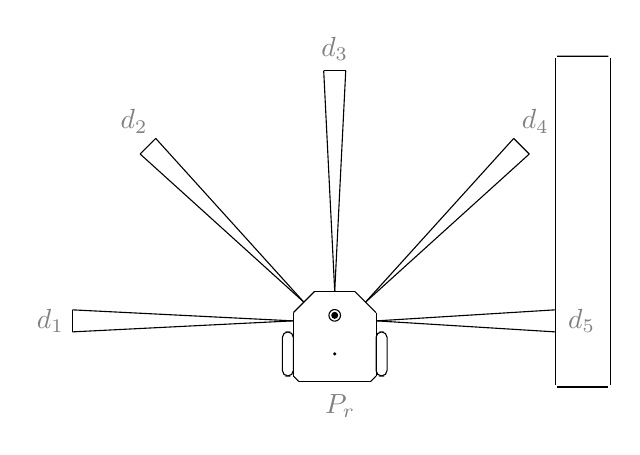
\begin{tikzpicture}[scale = 1.4]%
			\meuRoboLindaoCompEO
			\desenharSensoresTriangulo
		\end{tikzpicture}%
		
		\label{fig:CompEOa}%
		\caption{Sensores infravermelho}%
	\end{subfigure}%
	~
	\begin{subfigure}[t]{0.5\textwidth}%
		\centering%
		
		\begin{tikzpicture}[scale = 1.4]%
			\meuRoboLindaoCompEO
			\desenharSensoresVetores
		\end{tikzpicture}%
			
		\label{fig:CompEOb}%
		\caption{Vetores utilizados}%
	\end{subfigure}%
	\\
	\textbf{Fonte: autoria própria}
\end{figure}
		
		É interessante definir sistemas de coordenadas para cada sensor de modo que a coordenada
		do obstáculo possa ser representada como um vetor da forma $[d_i\ 0]^T$, onde $d_i$ é a 
		distância detectada pelo i-ésimo sensor. Assim, a representação é extremamente simples
		e, com matrizes de rotação, pode-se encontrar suas posições no sistemas de coordenadas
		do robô. 
		
		A representação dos obstáculos no sistema de coordenadas do robô está retratada na 
		Equação \ref{eq:ao_robot_frame}, onde $\theta_i$ é o ângulo do i-ésimo sensor, $d_i$ é a 
		distância ao obstáculo (pode estar saturada) e $[o_x\ o_y]_i^T$ é um vetor na coordenada
		do robô que define um \textit{offset}, apontando para a origem do sistema de coordenadas
		do sensor.
		\begin{equation}
			\label{eq:ao_robot_frame}
			\mleft[ 
			\begin{array}{c c}
				x \\ y
			\end{array}
			\mright]_i^R = \mleft[
			\begin{matrix}
		  		\cos{\theta_i} & -\sin{\theta_i} \\
		  		\sin{\theta_i} & \cos{\theta_i} \\
			\end{matrix}
			\mright] \mleft[ 
			\begin{array}{c c}
				d_i \\ 0
			\end{array}
			\mright] + \mleft[ 
			\begin{array}{c c}
				o_x \\ o_y
			\end{array}
			\mright]_i^R
		\end{equation}

		Os cinco sensores foram posicionados de modo a formar ângulos de $-\pi/2$, $-\pi/4$,
		$0$, $\pi/4$ e $\pi/2$, respectivamente. Os cinco vetores no sistema de coordenadas do 
		robô são combinados linearmente para formar uma única recomendação. A recomendação é 
		dada pela Equação \ref{eq:eo_comb_linear}, onde os vetores $v_1$ a $v_5$ são os mesmos 
		da Figura \ref{fig:CompEO}.b, os valores $k_1$ a $k_5$ são constantes e o vetor $v_{eq}$ 
		é um vetor arbitrário cuja escolha será explicada.
		\begin{equation}
			\label{eq:eo_comb_linear}
			\mathbf{u_{eo1}} = k_1 \mathbf{v_1} + k_2 \mathbf{v_2} + k_3 \mathbf{v_3} + 
			k_4 \mathbf{v_4} + k_5 \mathbf{v_5} + \mathbf{v_{eq}}
		\end{equation}
		
		As constantes $k_1$ a $k_5$ valem respectivamente, 0.7, 2, 1.2, 2 e 0.7. Elas
		foram definidas a partir de simulação. A razão de considerar peso maior para os sensores
		diagonais ($-\pi/4$ e $\pi/4$) é causar uma deflexão ao encontrar obstáculos frontais. 
		O peso pequeno nos sensores laterais ($-\pi/2$ e $\pi/2$) é devido ao baixo risco de 
		colisão, já que o sentido de movimento do robô é perpendicular a estes obstáculos.
		
		Em condição de ausência de obstáculos, os módulos dos vetores $v_1$ a $v_5$ estarão 
		saturados em 80 (cálculo dos sensores em centímetros). Neste caso, a soma dos cinco 
		primeiros termos tem como resultante um vetor ao longo do eixo X no sistema de 
		coordenadas do robô. Ao encontrar uma parede posicionada na perpendicular em relação 
		ao sentido de movimento, a resultante continuaria no eixo X (no sistema de coordenadas 
		do robô), provocando colisão. 
		O vetor $\mathbf{v_{eq}}$ tem por objetivo reduzir a magnitude da resultante. Seu
		módulo poderia ser definido de modo que a resultante se torne zero a uma distância 
		segura do obstáculo. 
		
		A condição de equilíbrio é indesejável, pois o robô não atinge o objetivo, mas 
		este caso é um excelente ponto de partida para compreender o comportamento
		de evitar obstáculo. A partir do equilibrio, se for adicionado um obstáculo à frente de
		qualquer sensor (ou se um obstáculo já existente for aproximado), a magnitude do vetor
		correspondente diminui, e a resultante será no sentido contrário.
		
		O valor de $\mathbf{v_{eq}}$ foi definido como $[-240 \ 0]^T$ (unidade em centímetros), 
		de modo que o robô não para até se chocar com o obstáculo. Portanto, o efeito deste 
		vetor é apenas reduzir a aparente ``inércia'' e aumentar o efeito de deflexão ao 
		encontrar obstáculos em ângulos oblíquos. 
		
		Para aproximações com angulos retos, é necessário um cálculo distinto, que afaste a 
		resultante do eixo x (no sistema de coordenadas do robô). Para este fim, o vetor da 
		Equação \ref{eq:eo_comb_linear2} é rotacionado. Como este é um caso emergencial, pela
		iminência de colisão, a recomendação de velocidade linear é zerada, de modo que na
		etapa de conversão entre modelo uniciclo e modelo de acionamento diferencial, a saída
		é uma rotação pura, que dura apenas o suficiente para o obstáculo ser percebido como 
		obliquo e o cálculo da Equação \ref{eq:eo_comb_linear} voltar a ser adotado. 
		\begin{equation}
			\label{eq:eo_comb_linear2}
			\mathbf{u_{eo2}} = k_1 \mathbf{v_1} + k_2 \mathbf{v_2} + k_3 \mathbf{v_3} + 
			k_4 \mathbf{v_4} + k_5 \mathbf{v_5}
		\end{equation}
		
		O cálculo final para a recomendação ``Evitar Obstáculo" é dado pela Equação 
		\ref{eq:eo_comb_linear3}, onde $D_{insegura}$ vale 25 centímetros. Essa recomendação 
		é no sistema de coordenadas do robô e deve ser convertida para o sistema global antes 
		de continuar os cálculos.
		\begin{equation}
			\label{eq:eo_comb_linear3}
			\mathbf{u_{eo}} = 
			\begin{cases}
				\mathbf{u_{eo1}} & \text{para} \ | \mathbf{v_3} | \geq D_{insegura} \\
				
				\mleft[
				\begin{matrix}
		  			\cos{(90)} & -\sin{(90)} \\
		  			\sin{(90)} & \cos{(90)} \\
				\end{matrix}
				\mright] \mathbf{u_{eo2}} & 				
				\begin{matrix*}[l]
		  			\text{para} \ | \mathbf{v_3} | < D_{insegura} \ \land \\
		  			k_1 \ (|\mathbf{v_5}| - |\mathbf{v_1}|) + k_2 \ (|\mathbf{v_4}| - |\mathbf{v_2}|)
					> 0 \\
				\end{matrix*} \\
				
				\mleft[
				\begin{matrix}
		  			\cos{(-90)} & -\sin{(-90)} \\
		  			\sin{(-90)} & \cos{(-90)} \\
				\end{matrix}
				\mright] \mathbf{u_{eo2}} & 
				\begin{matrix*}[l]
		  			\text{para} \ | \mathbf{v_3} | < D_{insegura} \ \land \\
		  			k_1 \ (|\mathbf{v_5}| - |\mathbf{v_1}|) + k_2 \ (|\mathbf{v_4}| - |\mathbf{v_2}|)
					\leq 0 \\
				\end{matrix*} \\
			\end{cases}
		\end{equation}
		
		O controlador PID para comportamento ``Evitar Obstáculo'' é calculado do mesmo modo
		que no comportamento ``Ir Para Objetivo''.
		
		\subsubsection{Comportamento mesclado ``Ir Para Objetivo e Evitar Obstáculo''}
		
		Situações de transição entre comportamentos podem trazer problemas que foram discutidos 
		na Seção \ref{SEC:SISTEMASHIBRIDOS}. Uma forma de mitigar possíveis oscilações é por meio da definição de um novo 
		comportamento em uma região intermediária entre as duas regiões (verificar 
		Figura \ref{fig:Sliding}).
		
		Vale salientar que um novo comportamento não resolve o problema, pois passam a existir 
		duas fronteiras ao invés de uma. Contudo, se este novo comportamento for definido como 
		combinação linear entre vetores das regiões vizinhas, as transições se vistas separadamente
		provocam mudanças mais suaves nas recomendações, o que é capaz de mitigar oscilações.
		
		Essa abordagem é escalável, no sentido de que para cada fronteira, um novo comportamento
		pode ser criado. A ideia aqui é que, com infinitas iterações, um sistema vetorial 
		descontínuo se tornaria um sistema contínuo.
		
		Neste caso apenas uma iteração foi necessária e o cálculo pode ser visto na Equação 
		\ref{eq:eo_e_ipo}, onde k vale 0,3. O vetor $\hat{\mathbf{u}}_{ipo}$ é o mesmo definido
		na Subseção \ref{SEC:IPO}, porém normalizado e o vetor $\hat{\mathbf{u}}_{eo}$ é da 
		Equação \ref{eq:eo_comb_linear}, também normalizado e convertido para o sistema de
		coordenadas global.		
		\begin{equation}
			\label{eq:eo_e_ipo}
			\mathbf{u_{eo\_e\_ipo}} = k \ \hat{\mathbf{u}}_{ipo} + (1-k) \ \hat{\mathbf{u}}_{eo}
		\end{equation}
		
		O controlador PID para comportamento ``Ir Para Objetivo e Evitar Obstáculo'' é calculado 
		do mesmo modo que nos comportamentos apresentados anteriormente.
		
		\subsubsection{Mínimos locais}
		
		Como a arquitetura comportamental é baseada em campos vetoriais (e ainda descontínuos),
		mínimos locais, quando presentes, podem fazer o robô nunca alcançar um objetivo. 
		
		A figura \ref{fig:CompSP} mostra diferentes tipos de obstáculos, a fim de discutir 
		suas interações com um robô que utilize apenas comportamentos ``Ir Para Objetivo" (IPO) e 
		``Evitar Obstáculo" (EO). Um robô que se dirige ao objetivo tem o comportamento IPO ativo
		e ao encontrar um obstáculo muda o comportamento para EO. 
		
		\newcommand{\meuRoboLindaoCompMinimos}{
	\begin{scope}[shift={(0,0.3)}]
		% Pr 
		\begin{scope}[shift={(0,-0.3)}, scale = 0.5]
			\node[color = gray] at (0.1,-0.35) {$P_r$};
		\end{scope}
		\begin{scope}[rotate=90,scale=0.5]
			\filldraw (0,0) circle (0.5pt);
			\begin{scope}[shift={(0.25,0)},rotate = -90]
				\RoboDiffClean
			\end{scope}
		\end{scope}
	\end{scope}
}%

\newcommand{\obstaculoA}[2]{
	\node[inner sep = 0pt] (P1) at (#1,0) {};
	\node[inner sep = 0pt] (P2) at (\fpeval{#1+(#2/2)},\fpeval{#2*sqrt{2}/2}) {};
	\node[inner sep = 0pt] (P3) at (\fpeval{#1+((3*#2)/2)},\fpeval{#2*sqrt{2}/2}) {};
	\node[inner sep = 0pt] (P4) at (\fpeval{#1+2*#2},0) {};
	\node[inner sep = 0pt] (P5) at (\fpeval{#1+((3*#2)/2)},\fpeval{-(#2*sqrt{2}/2)}) {};
	\node[inner sep = 0pt] (P6) at (\fpeval{#1+(#2/2)},\fpeval{-(#2*sqrt{2}/2)}) {};
	
	\draw[color = darkgray] (P1) -- (P2);
	\draw[color = darkgray] (P2) -- (P3);
	\draw[color = darkgray] (P3) -- (P4);
	\draw[color = darkgray] (P4) -- (P5);
	\draw[color = darkgray] (P5) -- (P6);
	\draw[color = darkgray] (P6) -- (P1);
	
	\node[color = gray] at (#1+#2,-1.3) {Obstáculo 1};
}

\newcommand{\obstaculoB}[3]{
	\node[inner sep = 0pt] (P1) at (#1,#2) {};
	\node[inner sep = 0pt] (P2) at (#1,#2+0.5) {};
	\node[inner sep = 0pt] (P3) at (#1+#3+0.5,#2+0.5) {};
	\node[inner sep = 0pt] (P4) at (#1+#3+0.5,-#2-0.5) {};
	
	\node[inner sep = 0pt] (P5) at (#1,-#2-0.5) {};
	\node[inner sep = 0pt] (P6) at (#1,-#2) {};
	\node[inner sep = 0pt] (P7) at (#1+#3,-#2) {};
	\node[inner sep = 0pt] (P8) at (#1+#3,#2) {};
	
	\draw[color = darkgray] (P1) -- (P2);
	\draw[color = darkgray] (P2) -- (P3);
	\draw[color = darkgray] (P3) -- (P4);
	\draw[color = darkgray] (P4) -- (P5);
	\draw[color = darkgray] (P5) -- (P6);
	\draw[color = darkgray] (P6) -- (P7);
	\draw[color = darkgray] (P7) -- (P8);
	\draw[color = darkgray] (P8) -- (P1);
	
	\node[color = gray] at (#1+0.25+#3/2,-2.8) {Obstáculo 2};
}

\newcommand{\obstaculoC}[2]{
	\node[inner sep = 0pt] (P1) at (#1,#2+0.5) {};
	\node[inner sep = 0pt] (P2) at (#1+0.5,#2+0.5) {};
	\node[inner sep = 0pt] (P3) at (#1+0.5,-#2-0.5) {};
	\node[inner sep = 0pt] (P4) at (#1,-#2-0.5) {};
	
	\draw[color = darkgray] (P1) -- (P2);
	\draw[color = darkgray] (P2) -- (P3);
	\draw[color = darkgray] (P3) -- (P4);
	\draw[color = darkgray] (P4) -- (P1);
	
	\node[color = gray] at (#1+0.25,-2.8) {Obstáculo 3};
}

\begin{figure}[ht]
	\centering%
	\caption{Tipos de obstáculos}%
	\label{fig:CompSP}%
		
	\begin{tikzpicture}[scale = 1.4]%
		% Robô
		\begin{scope}[rotate=-90]
			\meuRoboLindaoCompMinimos
		\end{scope}
		\obstaculoA{2}{1.5}
		\obstaculoB{4}{2}{2}
		\obstaculoC{8}{2}
		
		\begin{scope}[shift={(10,0)}]
			\filldraw (0,0) circle (1.5pt);
			\node[color = gray] at (0,-0.35) {Objetivo};
		\end{scope}
	\end{tikzpicture}%

	\textbf{Fonte: autoria própria}
\end{figure}
		
		Se encontrar o Obstáculo 1 (convexo), o robô adota o comportamento EO e ocorre uma deflexão
		em seu movimento. Quando não puder mais detectar obstáculos, o comportamento IPO volta ao 
		controle. O robô é capaz de contornar obstáculos desde que a deflexão não leve o 
		robô para uma posição em que ele já esteve (neste caso, o robô oscila entre os mesmos 
		comportamentos e visita as mesmas regiões indefinidamente). 
		
		O Obstáculo 2, por ser côncavo, ilustra melhor a situação de mínimo local. A deflexão 
		provocada pelo comportamento EO evita o obstáculo, mas visita uma região já conhecida. 
		Portanto o robô se aproxima e se afasta do obstáculo indefinidamente, vagando pela região
		de mínimo local. 
		 
		O Obstáculo 3 é um exemplo convexo com mínimo local. Na ausência de obstáculos, o vetor 
		do comportamento IPO diminui em magnitude à medida que o robô avança. Se este 
		comportamento leva a uma posição em que um obstáculo é simétrico em relação à linha entre 
		Robô e Objetivo, qualquer deflexão causada pelo comportamento EO é seguida de uma nova 
		aproximação, pois o vetor IPO terá um componente no sentido no eixo de simetria. 
		
		É necessário introduzir um comportamento capaz de afastar o robô de um mínimo local 
		detectado e este comportamento deve interagir com os anteriores de modo a não criar 
		novos mínimos locais. Neste caso, foi criado o comportamento ``Seguir Parede''.
		
		\subsubsection{Comportamento ``Seguir parede''}
		
		O comportamento ``Seguir Parede'' tem por intuito contornar obstáculos até retirar o robô 
		de uma região de mínimo local. A detecção de que o robô entrou em um mínimo local ou saiu 
		dele é papel do autômato e será discutido em outra seção. Aqui, parte-se do princípio de 
		que o robô com certeza está próximo a uma parede, na iminência de retornar a uma região 
		já visitada. A escolha de contornar no sentido horário ou anti-horário também fica a 
		cargo do autômato. 
		
		A Figura \ref{fig:CompSP} mostra dois casos de interesse para compreender o comportamento
		``Seguir Parede''. Como pode ser verificado, a detecção da parede utiliza sempre dois 
		sensores, pois com dois pontos, forma-se uma reta. Contudo, a escolha é feita entre três
		sensores. Quando é decidido contornar obstáculo no sentido anti-horário, os três sensores
		escolhidos são do sensor frontal ao sensor esquerdo e, para o sentido horário de contorno,
		os sensores vão do sensor frontal ao sensor direito.
		
		\newcommand{\meuRoboLindaoCompSP}{
	\begin{scope}[shift={(0,0.3)}]
		% Pr 
		\begin{scope}[shift={(0,-0.3)}, scale = 0.5]
			\node[color = gray] at (0.1,-0.35) {$P_r$};
		\end{scope}
		\begin{scope}[rotate=90,scale=0.5]
			\filldraw (0,0) circle (0.5pt);
			\begin{scope}[shift={(0.25,0)},rotate = -90]
				\RoboDiffClean
			\end{scope}
		\end{scope}
	\end{scope}
}%

\newcommand{\parede}[2]{
	\node[inner sep = 0pt] (P1) at (0,0) {};
	\node[inner sep = 0pt] (P2) at (#2,0) {};
	\node[inner sep = 0pt] (P3) at (#2,0.5) {};
	\node[inner sep = 0pt] (P4) at (0.5,0.5) {};
	\node[inner sep = 0pt] (P5) at (0.5,#1) {};
	\node[inner sep = 0pt] (P6) at (0,#1) {};
	\draw[color = darkgray] (P1) -- (P2);
	\draw[color = darkgray] (P2) -- (P3);
	\draw[color = darkgray] (P3) -- (P4);
	\draw[color = darkgray] (P4) -- (P5);
	\draw[color = darkgray] (P5) -- (P6);
	\draw[color = darkgray] (P6) -- (P1);
}

\newcommand{\sensorVisaoTriangularSp}[1]{
	\draw[color = gray] (0,0) -- (-0.1,#1);
	\draw[color = gray] (0,0) -- (0.1,#1);
	\draw[color = gray] (-0.1,#1) -- (0.1,#1);
}

\newcommand{\sensorVisaoVetorSp}[1]{
	\draw[->] (0,0) -- (0,#1);
}

\newcommand{\desenharSensoresTrianguloSPa}{
	\begin{scope}[shift={(0.38,0.6)},rotate=-90]
		\sensorVisaoTriangularSp{2}
	\end{scope}
	\begin{scope}[shift={(-0.38,0.6)},rotate=90]
		\sensorVisaoTriangularSp{2-1.3}
	\end{scope}
	\begin{scope}[shift={(0.28,0.77)},rotate=-45]
		\sensorVisaoTriangularSp{2}
	\end{scope}
	\begin{scope}[shift={(-0.28,0.77)},rotate=45]
		\sensorVisaoTriangularSp{2}
	\end{scope}	
	\begin{scope}[shift={(0,0.87)},rotate=0]
		\sensorVisaoTriangularSp{2}
	\end{scope}
}

\newcommand{\desenharSensoresTrianguloSPb}{
	\begin{scope}[shift={(0.38,0.6)},rotate=-90]
		\sensorVisaoTriangularSp{2-0.9}
	\end{scope}
	\begin{scope}[shift={(-0.38,0.6)},rotate=90]
		\sensorVisaoTriangularSp{2}
	\end{scope}
	\begin{scope}[shift={(0.28,0.77)},rotate=-45]
		\sensorVisaoTriangularSp{2-0.5}
	\end{scope}
	\begin{scope}[shift={(-0.28,0.77)},rotate=45]
		\sensorVisaoTriangularSp{2}
	\end{scope}	
	\begin{scope}[shift={(0,0.87)},rotate=0]
		\sensorVisaoTriangularSp{2-1}
	\end{scope}
}

\newcommand{\desenharLinhasParedeA}{
	\begin{scope}[shift={(-0.38,0.6)},rotate=90]
		\begin{scope}[shift={(0,2-1.3)}]
			\node[inner sep = 0pt] (P1) at (0,0) {};
		\end{scope}
	\end{scope}
	\begin{scope}[shift={(-0.28,0.77)},rotate=45]
		\begin{scope}[shift={(0,2)}]
			\node[inner sep = 0pt] (P2) at (0,0) {};
		\end{scope}
	\end{scope}
	
	\draw (P1) -- (P2);
}

\newcommand{\desenharLinhasParedeB}{
	\begin{scope}[shift={(0.38,0.6)},rotate=-90]
		\begin{scope}[shift={(0,2-0.9)}]
			\node[inner sep = 0pt] (P1) at (0,0) {};
		\end{scope}
	\end{scope}
	\begin{scope}[shift={(0,0.87)},rotate=0]
		\begin{scope}[shift={(0,2-1)}]
			\node[inner sep = 0pt] (P2) at (0,0) {};
		\end{scope}
	\end{scope}
	
	\draw (P1) -- (P2);
}

\begin{figure}[ht]
	\centering%
	\caption{Comportamento Seguir Parede}%
	\label{fig:CompSP}%
	\begin{subfigure}[t]{0.5\textwidth}%
		\centering%
		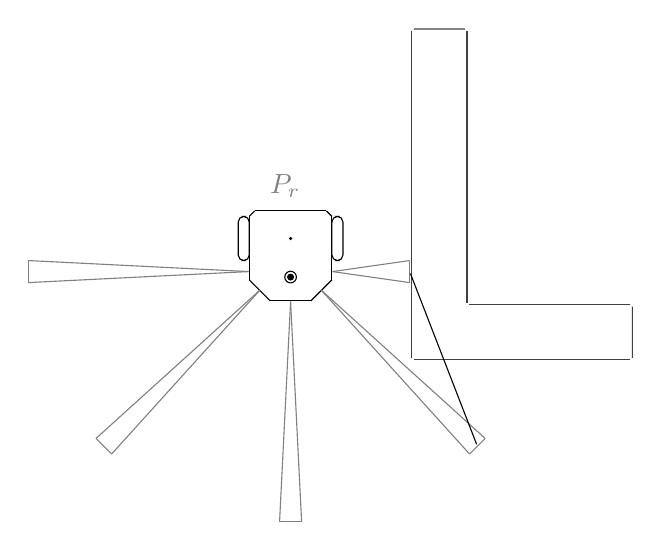
\begin{tikzpicture}[scale = 1.4]%
			% Obstáculo
			\parede{3}{2}
			% Robô
			\begin{scope}[shift={(-1.1,1.4)},rotate=180]
				\meuRoboLindaoCompSP
				\desenharSensoresTrianguloSPa
				\desenharLinhasParedeA
			\end{scope}
		\end{tikzpicture}%
		
		\label{fig:CompSPa}%
		\caption{Parede subestimada}%
	\end{subfigure}%
	~
	\begin{subfigure}[t]{0.5\textwidth}%
		\centering%
		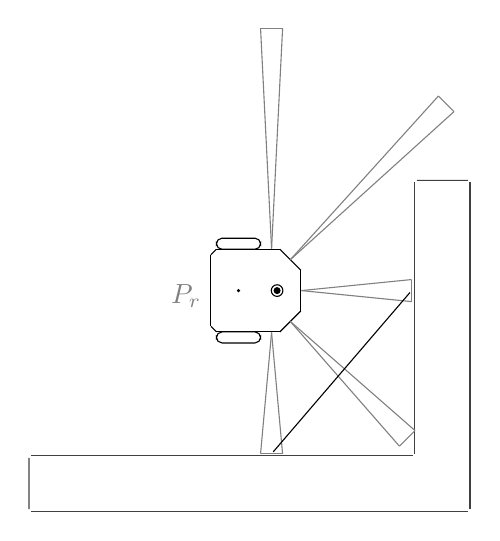
\begin{tikzpicture}[scale = 1.4]%
			% Obstáculo
			\begin{scope}[shift={(0,0)},xscale=-1,yscale=1]
				\parede{3}{4}
			\end{scope}
			% Robô
			\begin{scope}[shift={(-2.4,2)},rotate=-90]
				\meuRoboLindaoCompSP
				\desenharSensoresTrianguloSPb
				\desenharLinhasParedeB
			\end{scope}
		\end{tikzpicture}%
			
		\label{fig:CompSPb}%
		\caption{Parede superestimada}%
	\end{subfigure}%
	\\
	\textbf{Fonte: autoria própria}
\end{figure}
		
		Uma vez definidos os três sensores de interesse, a reta que descreve a parede é calculada 
		utilizando os dois sensores com menor valor de distância e, caso tenha empate, a 
		prioridade de escolha vai do sensor lateral ao frontal (lateral com a maior prioridade, 
		frontal com a menor). 
		
		É necessário mencionar que a simplificação da parede como reta pode subestimar ou 
		superestimar a parede real. A Figura \ref{fig:CompSP}.a é um caso de subestimativa, já 
		que o segmento de reta secciona a parede real. A Figura \ref{fig:CompSP}.b mostra uma 
		superestimativa, pois o segmento de reta está muito distante da parede real. A 
		superestimativa não é um problema grave, pois o robô não corre risco de colidir. 
		Subestimar a parede, por outro lado, leva a uma aproximação perigosa. Para evitar 
		colisão, é necessário definir uma distância segura para seguir parede. Com uma distância
		suficiente, a aproximação não traz risco de colisão.
		
		Na etapa seguinte do cálculo, parte-se de uma reta que descreve a parede e calcula-se um
		vetor a ser seguido. A Figura \ref{fig:CompSPVetor} ilustra essa etapa. 

		\newcommand{\desenharLinhasParedeC}[2]{
	\begin{scope}[shift={(-0.38,0.6)},rotate=90]
		\begin{scope}[shift={(0,2-1.3)}]
			\node[inner sep = 0pt] (P1) at (0,0) {};
		\end{scope}
	\end{scope}
	\begin{scope}[shift={(-0.28,0.77)},rotate=45]
		\begin{scope}[shift={(0,2)}]
			\node[inner sep = 0pt] (P2) at (0,0) {};
		\end{scope}
	\end{scope}
	
	\draw (P1) -- (P2);
	
	% linhas continuacao:
	\def\UserVetAX{-1.08}
	\def\UserVetAY{0.6}
	
	\def\UserVetXNum{\fpeval{-0.28-sqrt(2)+1.08}}
	\def\UserVetYNum{\fpeval{0.77+sqrt(2)-0.6}}
	\def\UserVetMod{\fpeval{sqrt(\UserVetXNum*\UserVetXNum + \UserVetYNum*\UserVetYNum)}}
	
	\def\UserVetX{\fpeval{\UserVetXNum/\UserVetMod}}
	\def\UserVetY{\fpeval{\UserVetYNum/\UserVetMod}}
	
	\def\UserLinhaTrasX{\fpeval{-1.08 -\UserVetX*#1}}
	\def\UserLinhaTrasY{\fpeval{0.6 -\UserVetY*#1}}
	\def\UserLinhaFrenteX{\fpeval{-0.28-sqrt(2) +\UserVetX*#2}}
	\def\UserLinhaFrenteY{\fpeval{0.77+sqrt(2) +\UserVetY*#2}}
			
	\draw [dashed] (P1) -- (\UserLinhaTrasX,\UserLinhaTrasY);
	\draw [dashed] (P2) -- (\UserLinhaFrenteX,\UserLinhaFrenteY);
	
	\def\distance{\fpeval{\UserVetX * \UserVetAX + \UserVetY * (\UserVetAY - 0.3)}}
	\begin{scope}[shift={(0,0.3)}]
		\def\UserVetPerpX{\fpeval{\UserVetAX-\distance*\UserVetX}}
		\def\UserVetPerpY{\fpeval{(\UserVetAY - 0.3)-\distance*\UserVetY}}
		\def\UserVetPerpNormX{\UserVetPerpX/(sqrt(\UserVetPerpX*\UserVetPerpX + \UserVetPerpY*\UserVetPerpY))}
		\def\UserVetPerpNormY{\UserVetPerpY/(sqrt(\UserVetPerpX*\UserVetPerpX + \UserVetPerpY*\UserVetPerpY))}
	
		\draw[-{Latex[length=2mm]}] (0,0) -- (P1) node [black,midway,yshift=-0.21cm,xshift=0.1cm] {$u_a$};
		\begin{scope}[shift={(P1)}]
			\draw[-{Latex[length=2mm]}] (0,0) -- (\UserVetX, \UserVetY) node [black,midway,xshift=-0.3cm,yshift=0.1cm] {$u_t$};
		\end{scope}
		\draw[-{Latex[length=2mm]}] (0,0) -- (\UserVetPerpX, \UserVetPerpY)
		node [black,midway,yshift=0.3cm,xshift=0.2] {$u_p$};

		\def\UserChavesX{\fpeval{\UserVetAX-\distance*\UserVetX}}
		\def\UserChavesY{\fpeval{(\UserVetAY - 0.3)-\distance*\UserVetY}}	
		\draw [decorate,decoration={brace,amplitude=10pt},xshift=-2pt,yshift=-2pt]
			(\UserChavesX, \UserChavesY) -- (\fpeval{-1.08},\fpeval{0.3}) 
			node [black,midway,xshift=0.6cm, yshift=0.1cm] {$d$};
			
		% angulo reto:
		\def\UserTamanhoQuad{0.15}
		\def\UserPontoEsqX{\fpeval{\UserVetPerpX - \UserTamanhoQuad*\UserVetPerpNormX}}
		\def\UserPontoEsqY{\fpeval{\UserVetPerpY - \UserTamanhoQuad*\UserVetPerpNormY}}
		\def\UserPontoDirX{\fpeval{\UserVetPerpX + \UserTamanhoQuad*\UserVetX}}
		\def\UserPontoDirY{\fpeval{\UserVetPerpY + \UserTamanhoQuad*\UserVetY}}
		\def\UserPontoBaixoX{\fpeval{\UserVetPerpX - \UserTamanhoQuad*\UserVetPerpNormX + \UserTamanhoQuad*\UserVetX}}
		\def\UserPontoBaixoY{\fpeval{\UserVetPerpY - \UserTamanhoQuad*\UserVetPerpNormY + \UserTamanhoQuad*\UserVetY}}
		
		\draw (\UserVetPerpX, \UserVetPerpY) -- (\UserPontoEsqX, \UserPontoEsqY);
		\draw (\UserVetPerpX, \UserVetPerpY) -- (\UserPontoDirX, \UserPontoDirY);
		\draw (\UserPontoEsqX, \UserPontoEsqY) -- (\UserPontoBaixoX, \UserPontoBaixoY);
		\draw (\UserPontoDirX, \UserPontoDirY) -- (\UserPontoBaixoX, \UserPontoBaixoY);
		
		\filldraw (\fpeval{\UserVetPerpX - \UserTamanhoQuad*\UserVetPerpNormX/2 + \UserTamanhoQuad*\UserVetX/2}, 
		\fpeval{\UserVetPerpY - \UserTamanhoQuad*\UserVetPerpNormY/2 + \UserTamanhoQuad*\UserVetY/2}) circle (0.5pt);
		
		% Ângulo vetor
		\begin{scope}[shift={(P1)}, rotate=180]
			\draw (0.3*\UserVetX,0.3*\UserVetY) arc (110:160:0.3);
			\node at (-0.35,0.25) {\footnotesize $\theta$};
		\end{scope}
	\end{scope}
}

\begin{figure}[ht]
	\centering%
	\caption{Recomendação vetorial}%
	\label{fig:CompSPVetor}%
	
	\begin{tikzpicture}[scale = 1.4]%
		% Obstáculo
		%\parede{3}{2}
		% Robô
		\begin{scope}[shift={(-1.1,1.4)},rotate=180]
			\meuRoboLindaoCompSP
			\desenharSensoresTrianguloSPa
			\desenharLinhasParedeC{3}{2}
		\end{scope}
	\end{tikzpicture}%
	\\
	\textbf{Fonte: autoria própria}
\end{figure}
		
		O vetor $\mathbf{u_t}$ é um vetor normalizado que está ao longo da reta. $\mathbf{u_a}$ 
		é um vetor conhecido, centrado na origem do sistema de coordenadas do robô e que leva ao 
		ponto associado a um dos sensores utilizado para o calculo da reta. $\mathbf{u_p}$ é
		perpendicular à reta e pode ser calculado a partir da Equação 
		\ref{eq:vetorPerpendicularSP3}, onde $d$ é a distância mostrada na figura.
		\begin{equation}
			\label{eq:vetorPerpendicularSP3}
			\mathbf{u_p} = \mathbf{u_a} - d \cdot \mathbf{u_t}
		\end{equation}
		
		O cálculo da distância $d$ é feito por produto escalar, A Equação 
		\ref{eq:vetorPerpendicularSP1} mostra essa operação, simplificada na Equação 
		\ref{eq:vetorPerpendicularSP2}. 
		\begin{equation}
			\label{eq:vetorPerpendicularSP1}
			\mathbf{u_a} \cdot \mathbf{u_t} = \mid \mathbf{u_a} \mid \cdot \mid \mathbf{u_t} \mid \cos(\theta)
		\end{equation}
		\begin{equation}
			\label{eq:vetorPerpendicularSP2}
			\mathbf{u_a} \cdot \mathbf{u_t} = \mid \mathbf{u_a} \mid \cos(\theta) = d
		\end{equation}
		
		A partir destes vetores, o vetor recomendação para o comportamento é dado pela Equação
		\ref{eq:calculoVetorFW}, onde $\beta$ é uma constante e $d_{fw}$ é a distância segura já
		citada anteriormente. 
		\begin{equation}
			\label{eq:calculoVetorFW}
			\mathbf{u_{fw}} = \mathbf{u_t} + \beta \cdot \left(\mathbf{u_p} - d_{fw} \cdot 
			\frac{\mathbf{u_p}}{\mid \mathbf{u_p} \mid}\right)
		\end{equation}
		
		O termo $(\mathbf{u_p} - d_{fw} \cdot \mathbf{u_p}/\mid\mathbf{u_p}\mid)$ é um vetor 
		perpendicular que aponta para uma linha paralela à parede, a uma distância $d_{fw}$. 
		Assim, se a distância entre robô e parede for diferente de $d_{fw}$, essa componente será 
		diferente de zero e seu efeito será no intuito de reduzir a diferença. A constante $\beta$
		serve para definir a importância do vetor perpendicular, já que $u_t$ é um vetor
		normalizado. Após simulação, o valor $\beta$ foi definido como 5,5. $d_{fw}$ foi definido
		como sendo 50 centímetros.
		
		O controlador para o comportamento ``Seguir Parede'' é apenas um controlador proporcional,
		pois o vetor referência muda constantemente. O termo derivativo, se utilizado de forma 
		inadequada (sem filtro, ou com valores altos para $k_d$), traz oscilações indesejadas. O 
		termo integrador é lento para entradas que variam muito. Uma constante $K_p = 2$ foi 
		utilizada, escolhida empiricamente, em simulação.
		
		\subsubsection{O autômato para arbitragem de comportamentos}
	
		Para o funcionamento do autômato, um último comportamento foi adicionado. O comportamento 
		``Parar'' apenas retira acionamento dos motores e deve assumir controle ao atingir o 
		objetivo.
		
		A Tabela \ref{tab:automatoEstados} mostra os comportamentos existentes. Os índices são
		os estados do autômato. 
	
		\begin{table}[ht]
\centering
\caption{Estados do autômato}
\vspace{0.2 cm}
\begin{tabular}{|c|l|l|}
\hline
Índice & Comportamento & Descrição                                         \\ \hline
0      & P             & Parar                                             \\ \hline
1      & IPO           & Ir para Objetivo                                  \\ \hline
2      & EO            & Evitar Obstáculos                                 \\ \hline
3      & IPO\_E\_EO    & Ir para Objetivo e Evitar Obstáculos (combinados) \\ \hline
4      & SP AH         & Seguir Parede sentido Anti-horário				   \\ \hline
5      & SP H          & Seguir Parede sentido Horário                     \\ \hline
\end{tabular}
\label{tab:automatoEstados}
\end{table}
	
		As funções de transição são formadas por condições, que foram resumidas na Tabela 
		\ref{tab:automatoEventos}. A tabela traz equações ou algoritmos para cálculo de cada 
		condição (saídas são ``verdadeiro'' ou ``falso'').
		
		\begin{table}[ht]
\centering
\caption{Condições utilizadas nas transições do autômato}
\vspace{0.2 cm}
\begin{tabular}{|c|l|l|}
\hline
Legenda & Condições                 & Cálculo da condição \\ \hline
a       & No objetivo               & Equacao1            \\ \hline
b       & Fez progresso             & Equacao1            \\ \hline
c       & Tem Obstáculo             & Equacao1            \\ \hline
d       & Está inseguro             & Equacao1            \\ \hline
e       & Livre de obstáculo        & Equacao1            \\ \hline
f       & Contornando pela esquerda & Equacao1            \\ \hline
g       & Contornando pela direita  & Equacao1            \\ \hline
\end{tabular}
\label{tab:automatoEventos}
\end{table}
		
		A condição ``no objetivo'' verifica se o objeto chegou ao objetivo. Seu cálculo pode
		ser visto na Equação \ref{eq:eventoNoObjetivo}, onde $\mathbf{v_{objetivo}}$ é o vetor 
		que aponta para o objetivo, $\mathbf{v_{\text{robô}}}$ é o vetor que aponta para a coordenada 
		do robô e $D_{STOP}$ é uma distância de tolerância, que foi definida como 15 centímetros. 
		Assim, atingir o objetivo é alcançar uma região circular de raio $D_{STOP}$.
		\begin{equation}
			\label{eq:eventoNoObjetivo}
			\mid \mathbf{v_{\text{objetivo}}} - \mathbf{v_{\text{robô}}} \mid < D_{STOP}
		\end{equation}
		
		A condição ``fez progresso'' tem por intuito detectar se o robô está avançando em 
		direção ao objetivo. Essa condição detecta entrada e saída de mínimos locais, já que, 
		parar de fazer progresso significa que o robô está retornando a região já visitada. Quando
		voltar a fazer progresso, significa que saiu de mínimo local. O Algoritmo 
		\ref{alg:fezProgresso} mostra o cálculo dessa função booleana. a variável $d_{prog}$ é a última distância 
		verificada e é atualizada no mesmo algoritmo. No início da navegação ou quando o objetivo
		for alterado, $d_{prog}$ deve ser inicializado para um valor infinito (no robô, foi usado 
		valor de 1000 metros, já que nunca será requisitado ao robô percorrer tal distância). A 
		constante $D_{PROG\_EPSILON}$ foi definida como 2 centímetros e seu intuito é não permitir
		que distâncias consideradas infinitesimais sejam consideradas como progresso.
		\begin{algorithm}
		\caption{Verificação de progresso}
		\label{alg:fezProgresso}%
		\begin{algorithmic}[1]
	
		\REQUIRE $d_{prog}, \mathbf{v_{\text{objetivo}}}, \mathbf{v_{\text{robô}}}$
		\ENSURE $d_{prog}, retornoBooleano$
	
		\IF{$\mid \mathbf{v_{\text{objetivo}}} - \mathbf{v_{\text{robô}}} \mid < (d_{prog} - D_{PROG\_EPSILON})$}
			\STATE $d_{prog} \leftarrow min(\mid \mathbf{v_{\text{objetivo}}} - \mathbf{v_{\text{robô}}} \mid, d_{prog})$
			\STATE $retornoBooleano \leftarrow Verdadeiro$
		\ELSIF{$abs(\mid \mathbf{v_{\text{objetivo}}} - \mathbf{v_{\text{robô}}} \mid - d_{prog}) \leq D_{PROG\_EPSILON}$}
			\STATE $retornoBooleano \leftarrow Verdadeiro$
		\ELSE
			\STATE $retornoBooleano \leftarrow Falso$ 
		\ENDIF
	
		\end{algorithmic}
		\end{algorithm}
	
		A condição ``tem obstáculo'' detecta se pelo menos algum sensor percebe existência de 
		obstáculo. A Equação \ref{eq:eventoTemObstaculo} mostra a função booleana, onde ``any''
		é o quantificador lógico ``algum'' que verifica se algum item no vetor $\mathbf{d_s}$ 
		(que especifica distância detectada pelos cinco sensores) cumpre a condição especificada, 
		de ser menor que a constante $D_{\text{EM\_OBSTÁCULO}}$, definida como 75 centímetros.
		\begin{equation}
			\label{eq:eventoTemObstaculo}
			any(\mathbf{d_s} < D_{\text{EM\_OBSTÁCULO}})
		\end{equation}
		
		A condição ``está inseguro'' detecta se algum sensor percebe a existência de obstáculo 
		em proximidade preocupante. A Equação \ref{eq:eventoEstaInseguro} mostra a função booleana.
		Neste caso, é verificado se algum item do vetor $\mathbf{d_s}$ é menor que uma constante 
		$D_{INSEGURO}$, definida como 25 centímetros.
		\begin{equation}
			\label{eq:eventoEstaInseguro}
			any(\mathbf{d_s} < D_{INSEGURO})
		\end{equation}
		
		A condição ``livre de obstáculo'' verifica se todos os sensores estão saturados, ou seja,
		sem obstáculos detectados. A Equação \ref{eq:eventoLivreObstaculo} mostra a função booleana,
		onde ``all'' é o quantificador lógico ``todos" que verifica se todos os itens do vetor 
		$\mathbf{d_s}$ cumprem a condição especificada no argumento (maior que 
		$D_{\text{EM\_OBSTÁCULO}}$). É importante salientar que ``livre de obstáculos'' não é 
		a negação de ``tem obstáculo'', apesar dos nomes. 
		\begin{equation}
			\label{eq:eventoLivreObstaculo}
			all(\mathbf{d_s} > D_{\text{EM\_OBSTÁCULO}})
		\end{equation}
				
		As condições ``contornando pela esquerda'' e ``contornando pela direita'' têm por intuito
		detectar se o robô está seguindo uma fronteira entre dois comportamentos em sentido 
		horário ou anti-horário, a fim a decidir o sentido em que adotará comportamento 
		``Seguir Parede''. Essa verificação no autômato ocorre junto com a condição ``não fez
		progresso'', de modo que, neste caso, os comportamentos ``Ir Para Objetivo'' e ``Evitar 
		Obstáculo'' estão em conflito (ângulo obtuso). 
		
		É desejável que o comportamento ``Seguir Parede'' escolhido esteja entre os dois 
		(similar ao que foi retratado na Figura \ref{fig:Sliding}). Então, por algebra linear, 
		deseja-se um vetor $\mathbf{u_{sp}} = \sigma_1 \cdot \mathbf{u_{ipo}} + \sigma_2 \cdot \mathbf{u_{eo}}$
		com constantes $\sigma_1$ e $\sigma_2$ maiores que zero. As Equações 
		\ref{eq:verificacaoSigma1} e \ref{eq:verificacaoSigma2} ilustram o cálculo dos valores 
		sigma. 
		\begin{equation}
			\label{eq:verificacaoSigma1}
			\left[\mathbf{u_{ipo}} \ \mathbf{u_{eo}}\right] 
			\mleft[ 
			\begin{array}{c c}
			\sigma_1 \\ \sigma_2
			\end{array}
			\mright]
			= \mathbf{u_{sp}}
		\end{equation}
		\begin{equation}
			\label{eq:verificacaoSigma2}
			\mleft[ 
			\begin{array}{c c}
			\sigma_1 \\ \sigma_2
			\end{array}
			\mright] = \left[\mathbf{u_{ipo}} \ \mathbf{u_{eo}}\right]^{-1} \cdot \mathbf{u_{sp}}
		\end{equation}
		  
		O algoritmo \ref{alg:sliding} calcula essas condições. A entrada ``sentidoDeContorno''
		define se o teste é para a condição ``contornando pela esquerda'' ou ``contornando pela
		direita''. As funções ``vetorIrParaObjetivo()'', ``vetorEvitarObstaculo()'' e 
		``vetorSeguirParede()'' calculam os vetores para os comportamentos ``Ir Para Objetivo'',
		``Evitar Obstáculo'' e ``Seguir Parede'', respectivamente. O último precisa do argumento
		``sentidoDeContorno'' para ser calculado. A função ``obstaculoPresente()'' verifica 
		apenas sensor lateral e diagonal (esquerdo ou direito dependendo do argumento) e retorna
		verdadeiro se algum deles não estiver saturado.
		\begin{algorithm}
		\caption{Verificação de situação de deslize em fronteira}
		\label{alg:sliding}%
		\begin{algorithmic}[1]
	
		\REQUIRE $sentidoDeContorno$
		\ENSURE $retornoBooleano$
	
		\STATE $u_{ipo, x}, u_{ipo, y} \leftarrow vetorIrParaObjetivo()$ 
		\STATE $u_{eo, x}, u_{eo, y} \leftarrow vetorEvitarObstaculo()$
		\STATE $u_{sp, x}, u_{sp, y} \leftarrow vetorSeguirParede(sentidoDeContorno)$
		
		\STATE $determinante \leftarrow u_{ipo, x} u_{ao, y} - u_{ipo, y} u_{ao, x}$
		\STATE $\sigma_1 \leftarrow (u_{ao, y} u_{sp, x} - u_{ao, x} u_{sp, y})/determinante$
		\STATE $\sigma_2 \leftarrow (-u_{ipo, y} u_{sp, x} + u_{ipo, x} u_{sp, y})/determinante$
		
		\IF{$obstaculoPresente(sentidoDeContorno) E \sigma_1 > 0 E \sigma_2 > 0$}
			\STATE $retornoBooleano \leftarrow Verdadeiro$
		\ELSE
			\STATE $retornoBooleano \leftarrow Falso$
		\ENDIF
	
		\end{algorithmic}
		\end{algorithm}
		
		A Figura \ref{fig:automatoHibrido} exibe o autômato completo. Suas transições serão 
		explicadas detalhadamente. 
		
		\tikzset{%
    block/.style={draw, fill=white, rectangle, 
            minimum height=2em, minimum width=3em},
    input/.style={inner sep=0pt},       
    output/.style={inner sep=0pt},      
    sum/.style = {draw, fill=white, circle, minimum size=2mm, node distance=1.5cm, inner sep=0pt},
    pinstyle/.style = {pin edge={to-,thin,black}}
}

\newcommand{\automatoHibrido}[1]{
\begin{tikzpicture}[scale = 1.1,->,auto ,node distance =4 cm and 5cm , on grid,
>=latex ,
state/.style ={scale = 1.1, circle, draw, minimum width =0.7cm},
finalstate/.style ={scale = 1.1, circle, draw, minimum width =0.7cm}]

	\node[state] (No3) {3};
	\begin{scope}[rotate=90]
		\begin{scope}[shift={(#1,0)}]
			\node[state] (No0) {0};
		\end{scope}
	\end{scope}
	\begin{scope}[rotate=90-72]
		\begin{scope}[shift={(#1,0)}]
			\node[state] (No5) {5};
		\end{scope}
	\end{scope}
	\begin{scope}[rotate=90-72*2]
		\begin{scope}[shift={(#1,0)}]
			\node[state] (No2) {2};
		\end{scope}
	\end{scope}
	\begin{scope}[rotate=90-72*3]
		\begin{scope}[shift={(#1,0)}]
			\node[state] (No1) {1};
		\end{scope}
	\end{scope}
	\begin{scope}[rotate=90-72*4]
		\begin{scope}[shift={(#1,0)}]
			\node[state] (No4) {4};
		\end{scope}
	\end{scope}
	
	\path[->] (No4) edge[bend left=20] node[xshift=-1cm, yshift=0.2cm] {$\neg a \land b \land \neg f$} (No3);
	\path[->] (No3) edge[bend left=20] node[xshift=1cm, yshift=-0.2cm] {$\neg a \land \neg b \land f$} (No4);
	\path[->] (No3) edge[bend left=20] node[xshift=1cm, yshift=0.2cm] {$\neg a \land \neg b \land g$} (No5);
	\path[->] (No5) edge[bend left=20] node[xshift=-0.1cm] {$\neg a \land b \land \neg g$} (No3);
	\path[->] (No3) edge[bend left=20] node[xshift=-0.9cm, yshift=1cm, rotate=-45] {$\neg a \land b \land \neg e \land d$} (No2);
	\path[->] (No2) edge[bend left=20] node[xshift=0.5cm, yshift=-0.6cm, rotate=-45] {$\neg a \land \neg d$} (No3);
	\path[->] (No3) edge[bend left=20] node {$a$} (No0);
	\path[->] (No0) edge[bend left=20] node {$\neg a$} (No3);
	\path[->] (No3) edge[bend left=20] node[xshift=-0.5cm, yshift=-0.6cm, rotate=45] {$\neg a \land b \land e$} (No1);
	\path[->] (No1) edge[bend left=20] node[xshift=0.2cm, yshift=0.3cm, rotate=45] {$\neg a \land b \land c$} (No3);
	
	\path[->] (No1) edge node {$\neg a \land b \land \neg c \land d$} (No2);
	\path[->] (No1) edge node[xshift=2.4cm, yshift=0.8cm] {$\neg a \land \neg b \land f$} (No4);
	\path[->] (No4) edge node {$a$} (No0);
	\path[->] (No5) edge node {$a$} (No0);
	
	\path[->,draw] (No1) .. controls ($(No2)+(1.5,-2)$) .. node[yshift=-0.2cm] {$\neg a \land \neg b \land g$} (No5);
	\path[->,draw] (No1) .. controls ($(No4)+(-2,1)$) .. node {$a$} (No0);
	\path[->,draw] (No2) .. controls ($(No5)+(2.1,1)$) .. node {$a$} (No0);
	
	% Input
	\coordinate[above = 1cm of No0, inner sep = 0pt] (input) {};
	\path[->] (input) edge (No0);
	
\end{tikzpicture}%
}

% Figura
\begin{figure}[ht]
	\centering
	\caption{Autômato Híbrido que soluciona o problema de navegação} 
	\label{fig:automatoHibrido}

	\automatoHibrido{5}
		
	\textbf{Fonte: autoria própria}
\end{figure}
		
		De todos os estados é possível chegar ao estado inicial ``Parar'' (0) por meio da 
		condição ``No Objetivo'' ($a$), mas para sair dele, uma redefinição de objetivo provoca
		a negação da condição de parada ($\neg a$) e o estado mesclado ``Ir para Objetivo e 
		Evitar Obstáculo'' (3) assume controle.
		
		A partir desse último, as transições para ``Seguir Parede'' (4 e 5) dependem da condição 
		``Não Fez Progresso'' ($\neg b$), mas a escolha do sentido de contorno depende das
		condições ``contornando pela esquerda'' e ``contornando pela direita'' ($f$ e $g$). A partir
		dos estados 4 ou 5, o retorno para o estado 3 depende de não ter encontrado objetivo 
		($\neg a$), voltar a fazer progresso ($b$) e deixar a situação de seguir fronteira 
		($\neg f$ ou $\neg g$).
		
		O estado 3 pode alcançar ``Ir Para Objetivo'' (1) quando está ``livre de obstáculo'' ($e$)
		e retorna quando volta a ``ter obstáculo" ($c$). O estado 1 alcança ``Seguir Parede'' com
		as mesmas condições utilizadas a partir do estado 3.
		
		Os estados 1 e 3 podem alcançar ``Evitar Obstáculo'' (2) por meio da condição ``está
		inseguro'' ($d$), mas uma vez neste estado, só pode retornar ao estado 3, com condição de
		``não estar inseguro'' ($\neg d$).
		
	\subsection{Controle \textit{Fuzzy}}
	
	Nesta seção, pretende-se demonstrar um controlador simples capaz de solucionar 
	o problema de navegação, usando sistema \textit{fuzzy}. 

	Já que intuito é implementar fusão de comportamentos, cada comportamento adicionado deve 
	ser projetado pensando em sua interação com todos os já existentes, o que dificulta o projeto,
	pois, se existirem recomendações conflitantes com o novo comportamento, este deve ser capaz 
	de suprimí-las. Isso é uma limitação de arquitetura e não pode ser confundido com uma 
	limitação do sistema \textit{fuzzy}, já que ele poderia implementar a arquitetura de 
	arbitragem também. 
	
	O controlador fuzzy foi definido de modo a controlar o modelo de acionamento diferencial,
	ao invés do modelo uniciclo. O algoritmo para priorizar velocidade angular sobre 
	velocidade linear foi mantido, bem como a abordagem de representar comportamentos por 
	vetores, de modo que ``fundir'' comportamentos é apenas combiná-los linearmente. Todos
	os comportamentos discutidos têm seus cálculos realizados no sistema de coordenadas do robô.
	O sistema global só é necessário para cálculo de odometria.
	
	\subsubsection{Comportamento ``Ir Para Objetivo''}
	
	O comportamento ``Ir Para Objetivo'' tem o mesmo intuito da contraparte híbrida, porém, 
	como as saídas vetoriais são todas normalizadas, o cálculo de ``IPO'' é normalizado.
	
	Esse cálculo não necessita de um controlador \textit{fuzzy} para gerar recomendações. Como as 
	coordenadas do objetivo e robô são conhecidas, o cálculo é direto. A Equação 
	\ref{eq:vetor_ipo_fuzzy} mostra a normalização. A variável $e_\theta$ é calculada pela
	Equação \ref{eq:vetor_ipo} e o vetor $\mathbf{u_{ipo}}$ é da Equação 
	\ref{eq:vetor_ipo_calculo}.
	\begin{equation}
		\label{eq:vetor_ipo_fuzzy}
			\mathbf{u_{ipo,\mathit{fuzzy}}} = 
			\begin{cases}
				\mleft[
				\begin{matrix}
		  			cos(e_\theta) \\
		  			sin(e_\theta) \\
				\end{matrix}
				\mright] & \text{, para} \ | \mathbf{u_{ipo}} | \geq 1 \\
				| \mathbf{u_{ipo}} | \cdot \mleft[
				\begin{matrix}
		  			cos(e_\theta) \\
		  			sin(e_\theta) \\
				\end{matrix}
				\mright] & \text{, para} \ | \mathbf{u_{ipo}} | < 1 \\
			\end{cases}
	\end{equation}
	
	\subsubsection{Comportamento ``Evitar Obstáculo''}
	
	O comportamento ``Evitar Obstáculo'' é semelhante à contraparte híbrida. O diagrama do
	controlador \textit{fuzzy}, relacionando entradas e saídas, pode ser visto na Figura 
	\ref{fig:fuzzyDiagramaEO}, onde as entradas ``SE'', ``SD'', ``SDE'', ``SDD'' e ``SF'' são
	valores para ``Sensor Esquerdo'', ``Sensor Direito'', ``Sensor Diagonal Esquerdo'', 
	``Sensor Diagonal Direito'' e ``Sensor Frontal'', respectivamente. As saídas ``RecYSE'',
	``RecYSD'', ``RecYSDE'', ``RecYSDD'', ``RecXSF'' são recomendações vetoriais, onde X ou Y
	especifica o eixo e os sufixos ``SE'', ``SD'', ``SDE'', ``SDD'' e ``SF'' indicam o sensor
	responsável pela recomendação. ``RecV'' é a recomendação para ``Velocidade linear''.
	
	\tikzset{%
    block/.style={scale = 1.2, draw, fill=white, rectangle, 
            minimum height=2em, minimum width=3em},
    input/.style={inner sep=0pt},       
    output/.style={inner sep=0pt},      
    sum/.style = {scale = 1.2, draw, fill=white, circle, minimum size=2mm, node
    distance=1.5cm, inner sep=0pt},
    pinstyle/.style = {scale = 1.2, pin edge={to-,thin,black}}
}

\begin{figure}[h]%
    \caption{Diagrama do sistema \textit{Fuzzy} ``Evitar Obstáculo''}%
    \centering
    
\begin{tikzpicture}[scale = 1.2, auto, node distance=2cm, on grid,
>=latex']%
	\node[block] (SE) {SE};
	\node[block, below = 1.4cm of SE] (SD) {SD};
	\node[block, below = 1.4cm of SD] (SDE) {SDE};
	\node[block, below = 1.4cm of SDE] (SDD) {SDD};
	\node[block, below = 1.4cm of SDD] (SF) {SF};
	
	\node[block, right = 6cm of SDE] (EO) {Evitar Obstáculo};
	
	\node[block, right = 6cm of EO, yshift = 0.7cm] (RecYSDE) {RecYSDE};
	\node[block, above = 1.4cm of RecYSDE, xshift=-0.2cm] (RecXSDE) {RecXSDE};
	\node[block, above = 1.4cm of RecXSDE, xshift=-0.2cm] (RecYSD) {RecYSD};
	\node[block, above = 1.4cm of RecYSD, xshift=-0.2cm] (RecYSE) {RecYSE};
	\node[block, below = 1.4cm of RecYSDE] (RecXSDD) {RecXSDD};
	\node[block, below = 1.4cm of RecXSDD, xshift=-0.2cm] (RecYSDD) {RecYSDD};
	\node[block, below = 1.4cm of RecYSDD, xshift=-0.2cm] (RecXSF) {RecXSF};
	\node[block, below = 1.4cm of RecXSF, xshift=-0.2cm] (RecV) {RecV};

	\draw [->] (SE) -- (EO);
	\draw [->] (SD) -- (EO);
	\draw [->] (SDE) -- (EO);
	\draw [->] (SDD) -- (EO);
	\draw [->] (SF) -- (EO);

	\draw [->] (EO) -- (RecYSE);
	\draw [->] (EO) -- (RecYSD);
	\draw [->] (EO) -- (RecXSDE);
	\draw [->] (EO) -- (RecYSDE);
	\draw [->] (EO) -- (RecXSDD);
	\draw [->] (EO) -- (RecYSDD);
	\draw [->] (EO) -- (RecXSF);
	\draw [->] (EO) -- (RecV);
\end{tikzpicture}%    
	
	\textbf{Fonte: autoria própria}
    \label{fig:fuzzyDiagramaEO}%
\end{figure}


	
	A partir das saídas do sistema \textit{fuzzy}, o vetor intermediário da Equação 
	\ref{eq:vetor_eo_fuzzy1} é calculado e o cálculo final para o Comportamento ``Evitar 
	Obstáculo'' é dado pela Equação \ref{eq:vetor_eo_fuzzy2}.
	\begin{equation}
		\label{eq:vetor_eo_fuzzy1}
			\mathbf{u_{eo,temp}} = 
			\mleft[
			\begin{matrix}
		  		2 \cdot RecXSF \\
		  		RecYSE + RecYSD + RecYSDE + RecYSDD \\
			\end{matrix}
			\mright]
	\end{equation}
	\begin{equation}
		\label{eq:vetor_eo_fuzzy2}
			\mathbf{u_{eo,\mathit{fuzzy}}} = 
			\begin{cases}
				\mathbf{u_{eo,temp}} & \text{, para} \ | \mathbf{u_{eo,temp}} | \leq 1 \\
				\frac{\mathbf{u_{eo,temp}}}{| \mathbf{u_{eo,temp}} |} & \text{, para} \ | \mathbf{u_{ipo}} | > 1 \\
			\end{cases}
	\end{equation}
	
	Os conjuntos \textit{fuzzy} utilizados para as entradas dos sensores estão retratados na
	Figura \ref{fig:fuzzyEOInput}, com as respectivas funções de pertinência. 
	
	\tikzset{%
    block/.style={draw, fill=white, rectangle, 
            minimum height=2em, minimum width=3em},
    input/.style={inner sep=0pt},       
    output/.style={inner sep=0pt},      
    sum/.style = {draw, fill=white, circle, minimum size=2mm, node distance=1.5cm, inner sep=0pt},
    pinstyle/.style = {pin edge={to-,thin,black}}
}

\begin{figure}[ht]%
    \caption{Conjuntos \textit{Fuzzy} para as entradas dos sensores}%
    \label{fig:fuzzyEOInput}%
    \centering
    
\begin{tikzpicture}[scale = 1, auto, node distance=2cm, on grid, >=latex']%
	\begin{axis}[xmin=0, xmax=0.8,ymax=1.1, samples=50, xlabel={distância},
	ylabel={$\mu$}, width=\textwidth, height=\axisdefaultheight, xtick distance={0.1}]
	
		\addplot [thick, color=black] table {
			0 0
			0.8 0
		};
		
		\addplot [thick, color=black] table {
			0 1
			0.4 0
		} node[color=gray, yshift=0.5cm, above, pos = .2] {DistP};
		
		\addplot [thick, color=black] table {
			0.1 0
			0.4 1
			0.7 0
		} node[color=gray, yshift=0.5cm, xshift=-0.1cm, above, pos = .4] {DistM};
		
		\addplot [thick, color=black] table {
			0.4 0 
			0.6 1
			0.8 0
		} node[color=gray, yshift=0.5cm, xshift=-0.2cm, above, pos = .4] {DistG};
		
		\addplot [thick, color=black] table {
			0.7 0
			0.8 1
		} node[color=gray, yshift=0.5cm, xshift=-0.6cm, above, pos = .8] {DistSat};
	\end{axis}
\end{tikzpicture}%
	
	\textbf{Fonte: autoria própria}
\end{figure}

	
	Já os conjuntos \textit{fuzzy} para saídas dos vetores associados a cada sensor, bem como 
	funções de pertinência, estão retratados na Figura \ref{fig:fuzzyEOOutputXY}. As saídas dos
	controladores \textit{fuzzy} estão sempre normalizadas.
	
	\tikzset{%
    block/.style={draw, fill=white, rectangle, 
            minimum height=2em, minimum width=3em},
    input/.style={inner sep=0pt},       
    output/.style={inner sep=0pt},      
    sum/.style = {draw, fill=white, circle, minimum size=2mm, node distance=1.5cm, inner sep=0pt},
    pinstyle/.style = {pin edge={to-,thin,black}}
}

\begin{figure}[!ht]%
    \caption{Conjuntos \textit{Fuzzy} para as saídas vetoriais}%
    \label{fig:fuzzyEOOutputXY}%
    \centering
    
\begin{tikzpicture}[scale = 1, auto, node distance=2cm, on grid, >=latex']%
	\begin{axis}[xmin=-1, xmax=1,ymax=1.1, samples=50, xlabel={Recomendação vetorial},
	ylabel={$\mu$}, width=\textwidth, height=\axisdefaultheight, 
	xtick distance={0.33333333333}, xticklabels={$$, $-1$, $-2/3$, $-1/3$, $0$, $1/3$, $2/3$, $1$}]
	
		\addplot [thick, color=black] table {
			-1 0
			1 0
		};
		
		\addplot [thick, color=black] table {
			-1 1
			-0.66666 0
		} node[color=gray, yshift=0.5cm, xshift=0.1cm, above, pos = .2] {NG};
		
		\addplot [thick, color=black] table {
			-1 0
			-0.66666 1
			-0.33333 0
		} node[color=gray, yshift=0.5cm, xshift=-0.1cm, above, pos = .4] {NM};
		
		\addplot [thick, color=black] table {
			-0.66666 0 
			-0.33333 1
			0 0
		} node[color=gray, yshift=0.5cm, xshift=-0.1cm, above, pos = .4] {NP};
		
		\addplot [thick, color=black] table {
			-0.33333 0 
			0 1
			0.33333 0
		} node[color=gray, yshift=0.5cm, xshift=-0.1cm, above, pos = .4] {Z};
		
		\addplot [thick, color=black] table {
			0 0 
			0.33333 1
			0.66666 0
		} node[color=gray, yshift=0.5cm, xshift=-0.1cm, above, pos = .4] {PP};
		
		\addplot [thick, color=black] table {
			0.33333 0 
			0.66666 1
			1 0
		} node[color=gray, yshift=0.5cm, xshift=-0.1cm, above, pos = .4] {PM};
		
		\addplot [thick, color=black] table {
			0.66666 0
			1 1
		} node[color=gray, yshift=0.5cm, xshift=-0.1cm, above, pos = .8] {PG};
	\end{axis}
\end{tikzpicture}%
	
	\textbf{Fonte: autoria própria}
\end{figure}

	
	Os conjuntos para a saída da recomendação em velocidade (``RecV''), bem como funções de
	pertinência, estão retratados na Figura \ref{fig:fuzzyEOOutputV}.
	
	\tikzset{%
    block/.style={draw, fill=white, rectangle, 
            minimum height=2em, minimum width=3em},
    input/.style={inner sep=0pt},       
    output/.style={inner sep=0pt},      
    sum/.style = {draw, fill=white, circle, minimum size=2mm, node distance=1.5cm, inner sep=0pt},
    pinstyle/.style = {pin edge={to-,thin,black}}
}

\begin{figure}[!ht]%
    \caption{Conjuntos \textit{Fuzzy} para a saída de velocidade}%
    \label{fig:fuzzyEOOutputV}%
    \centering
    
\begin{tikzpicture}[scale = 1, auto, node distance=2cm, on grid, >=latex']%
	\begin{axis}[xmin=0, xmax=1,ymax=1.1, samples=50, xlabel={Velocidade (normalizada)},
	ylabel={$\mu$}, width=\textwidth, height=\axisdefaultheight, 
	xtick distance={0.33333333333}, xticklabels={$$, $0$, $1/3$, $2/3$, $1$}]
	
		\addplot [thick, color=black] table {
			0 0
			1 0
		};
		
		\addplot [thick, color=black] table {
			0 0
			0.33333 1
			0.66666 0
		} node[color=gray, yshift=0.5cm, above, pos = .4] {VP};
		
		\addplot [thick, color=black] table {
			0.33333 0
			0.66666 1
			1 0
		} node[color=gray, yshift=0.5cm, above, pos = .4] {VM};
		
		\addplot [thick, color=black] table {
			0.66666 0
			1 1
		} node[color=gray, yshift=0.5cm, xshift=-0.1cm, above, pos = .8] {VG};
	\end{axis}
\end{tikzpicture}%
	
	\textbf{Fonte: autoria própria}
\end{figure}

	
	A Tabela \ref{tab:regrasEvitarObstaculo} mostra um conjunto de regras utilizado. Apesar de 
	ser um sistema MIMO (múltiplas entradas e multiplas saídas), poderia ser dividido em seis 
	sistemas com apenas uma saída, cada qual possuindo um menor conjunto de regras. Dado um 
	sensor específico, quando a distância mensurada é pequena, o vetor associado tem grande 
	magnitude e à medida que a distância tende à saturação, a magnitude do vetor associado 
	tende a zero. 
	
	\begin{table}[ht]
\caption{Regras \textit{Fuzzy} para sistema ``Evitar Obstáculo''}
\vspace{0.2 cm}
\resizebox{\linewidth}{!}{
\begin{tabular}{|c|c|c|c|c|c|c|c|c|c|c|c|}
\hline
\multirow{2}{*}{} & \multicolumn{5}{c|}{Entradas}                   & \multicolumn{6}{c|}{Saídas}                         \\ \cline{2-12} 
                  & SE      & SD      & SDE     & SDD     & SF      & RecYSE & RecYSD & RecYSDE & RecYSDD & RecXSF & RecV \\ \hline
1                 & DistP   & -       & -       & -       & -       & NG     & -      & -       & -       & -      & -    \\ \hline
2                 & DistM   & -       & -       & -       & -       & NM     & -      & -       & -       & -      & -    \\ \hline
3                 & DistG   & -       & -       & -       & -       & NP     & -      & -       & -       & -      & -    \\ \hline
4                 & DistSat & -       & -       & -       & -       & Z      & -      & -       & -       & -      & VG   \\ \hline
5                 & -       & DistP   & -       & -       & -       & -      & PG     & -       & -       & -      & -    \\ \hline
6                 & -       & DistM   & -       & -       & -       & -      & PM     & -       & -       & -      & -    \\ \hline
7                 & -       & DistG   & -       & -       & -       & -      & PP     & -       & -       & -      & -    \\ \hline
8                 & -       & DistSat & -       & -       & -       & -      & Z      & -       & -       & -      & VG   \\ \hline
9                 & -       & -       & DistP   & -       & -       & -      & -      & NG      & -       & -      & VP   \\ \hline
10                & -       & -       & DistM   & -       & -       & -      & -      & NM      & -       & -      & VM   \\ \hline
11                & -       & -       & DistG   & -       & -       & -      & -      & NP      & -       & -      & VM   \\ \hline
12                & -       & -       & DistSat & -       & -       & -      & -      & Z       & -       & -      & VG   \\ \hline
13                & -       & -       & -       & DistP   & -       & -      & -      & -       & PG      & -      & VP   \\ \hline
14                & -       & -       & -       & DistM   & -       & -      & -      & -       & PM      & -      & VM   \\ \hline
15                & -       & -       & -       & DistG   & -       & -      & -      & -       & PP      & -      & VM   \\ \hline
16                & -       & -       & -       & DistSat & -       & -      & -      & -       & Z       & -      & VG   \\ \hline
17                & -       & -       & -       & -       & DistP   & -      & -      & -       & -       & NG     & VP   \\ \hline
18                & -       & -       & -       & -       & DistM   & -      & -      & -       & -       & NM     & VM   \\ \hline
19                & -       & -       & -       & -       & DistG   & -      & -      & -       & -       & NP     & VM   \\ \hline
20                & -       & -       & -       & -       & DistSat & -      & -      & -       & -       & Z      & VG   \\ \hline
\end{tabular}
}
\label{tab:regrasEvitarObstaculo}
\end{table}
	
	Cada sensor pode ter no máximo dois ``valores ativos'' (pertinência maior que zero). Assim,
	para cinco entradas, pela tabela, teremos no máximo 10 regras ativas. 
	 
	\subsubsection{Comportamento ``Seguir parede''}

	O comportamento ``Seguir Parede'' também é necessário no controlador \textit{fuzzy} pela 
	questão dos mínimos locais, discutida anteriormente. Este deve assumir controle do robô 
	apenas quando necessário, suprimindo a tendência de retornar ao mínimo local. A necessidade 
	de uma hierarquia entre comportamentos motiva o uso da arquitetura de subsunção, discutida 
	brevemente na Seção \ref{SEC:SUBSUNCAO}.
	
	A Figura \ref{fig:fuzzyAtivacaoSubsuncao} mostra uma maneira simples de inibir 
	comportamentos. A função mostrada é responsável por definir o quão ativo o comportamento 
	``Seguir Parede'' está. Saída 0 significa totalmente inativo e saída 1 significa totalmente
	ativo. Uma combinação linear pode mesclar recomendações ativando ou desativando 
	comportamentos, dependendo do valor do coeficiente. 
	
	\tikzset{%
    block/.style={draw, fill=white, rectangle, 
            minimum height=2em, minimum width=3em},
    input/.style={inner sep=0pt},       
    output/.style={inner sep=0pt},      
    sum/.style = {draw, fill=white, circle, minimum size=2mm, node distance=1.5cm, inner sep=0pt},
    pinstyle/.style = {pin edge={to-,thin,black}}
}

\begin{figure}[ht]%
    \caption{Curva de Ativação para comportamento Seguir Parede}%
    \label{fig:fuzzyAtivacaoSubsuncao}%
    \centering
    
\begin{tikzpicture}[scale = 1, auto, node distance=2cm, on grid, >=latex']%
	\begin{axis}[xmin=0, xmax=40,ymax=1.1, samples=50, xlabel={Contador para Ativação},
	ylabel={Coeficiente}, width=\textwidth, height=\axisdefaultheight, 
	xtick distance={5}]
	
		\addplot [thick, color=black] table {
			0 0
			5 0
			35 1
			40 1
		};
	\end{axis}
\end{tikzpicture}%
	
	\textbf{Fonte: autoria própria}
\end{figure}

	
	A Figura \ref{fig:fuzzyDiagramaSP} mostra o diagrama do controlador, que associa entradas 
	e saídas. As entradas são as mesmas para o controlador ``Evitar Obstáculo''. As saídas
	``SPRecX'', ``SPRecY'', ``RegDistYSL'' e ``RegDistYSD'' são recomendações vetoriais. 
	``SPRecX'' é uma recomendação no eixo $x$ e ``SPRecY'' é recomendação ao longo de $y$. 
	``RegDistYSL'' e ``RegDistYSD'' tem por objetivo recomendar uma deflexão no eixo $y$, para
	que o robô siga a parede a uma distância segura. O sufixo ``SL'' designa que ``Sensores 
	Laterais'' são responsáveis pela recomendação, enquanto ``SD'' responsabiliza os 
	``Sensores Diagonais''. A distinção foi necessária para considerar pesos diferentes para
	sensores diagonais e laterais sem afetar outras saídas.
	
	\tikzset{%
    block/.style={scale = 1.2, draw, fill=white, rectangle, 
            minimum height=2em, minimum width=3em},
    input/.style={inner sep=0pt},       
    output/.style={inner sep=0pt},      
    sum/.style = {scale = 1.2, draw, fill=white, circle, minimum size=2mm, node
    distance=1.5cm, inner sep=0pt},
    pinstyle/.style = {scale = 1.2, pin edge={to-,thin,black}}
}

\begin{figure}[h]%
    \caption{Diagrama do sistema \textit{Fuzzy} ``Seguir Parede''}%
    \centering
    
\begin{tikzpicture}[scale = 1.2, auto, node distance=2cm, on grid,
>=latex']%
	\node[block] (SE) {SE};
	\node[block, below = 1.4cm of SE] (SD) {SD};
	\node[block, below = 1.4cm of SD] (SDE) {SDE};
	\node[block, below = 1.4cm of SDE] (SDD) {SDD};
	\node[block, below = 1.4cm of SDD] (SF) {SF};
	
	\node[block, right = 6cm of SDE] (SP) {Seguir Parede};
	
	\node[block, right = 6cm of SP, yshift = 0.7cm] (SPRecY) {SPRecY};
	\node[block, above = 1.4cm of SPRecY] (SPRecX) {SPRecX};
	\node[block, below = 1.4cm of SPRecY] (RegDistYSL) {RegDistYSL};
	\node[block, below = 1.4cm of RegDistYSL] (RegDistYSD) {RegDistYSD};

	\draw [->] (SE) -- (SP);
	\draw [->] (SD) -- (SP);
	\draw [->] (SDE) -- (SP);
	\draw [->] (SDD) -- (SP);
	\draw [->] (SF) -- (SP);

	\draw [->] (SP) -- (SPRecX);
	\draw [->] (SP) -- (SPRecY);
	\draw [->] (SP) -- (RegDistYSL);
	\draw [->] (SP) -- (RegDistYSD);
\end{tikzpicture}%    
	
	\textbf{Fonte: autoria própria}
    \label{fig:fuzzyDiagramaSP}%
\end{figure}


	
	A Equação \ref{eq:vetor_sp_fuzzy1} mostra o cálculo de um vetor temporário, definido a 
	partir das saídas do sistema \textit{fuzzy}. A constante ``C'' é o coeficiente de ativação
	e $\mathbf{u_{eo,fuzzy}}$ é a recomendação para ``Evitar Obstáculos'', que é somada
	de modo que mesmo que o comportamento ``SP'' esteja totalmente ativo, o robô ainda é capaz
	de evitar obstáculos. 
	\begin{equation}
		\label{eq:vetor_sp_fuzzy1}
			\mathbf{u_{sp,temp}} =
			\begin{cases}
			 
			\mleft[
			\begin{matrix}
		  		3 \cdot SPRecX \\
		  		RegDistYSL + 2,5 \cdot RegDistYSD + 2 \cdot SPRecY \\
			\end{matrix}
			\mright] + \mathbf{u_{eo,fuzzy}} & \text{, para} \ C > 0 \\
			
			\mleft[
			\begin{matrix}
		  		0 \\
		  		0 \\
			\end{matrix}
			\mright]  & \text{, para} \ C = 0 \\
			
			\end{cases}
	\end{equation}

	A recomendação \textit{fuzzy} para ``Seguir Parede'' (vetor $\mathbf{u_{sp,fuzzy}}$)
	é calculado pelo Algoritmo \ref{alg:RecSPFuzzy}. Cada função será discutida com detalhe. 
	\begin{algorithm}
		\caption{Cálculo Final da Recomendação ``Seguir Parede''}
		\label{alg:RecSPFuzzy}%
		\begin{algorithmic}[1]
	
		\ENSURE $\mathbf{u_{sp,\mathit{fuzzy}, x}}, \mathbf{u_{sp,\mathit{fuzzy}, y}}$
		
		\STATE $C \leftarrow verificaAtivacaoSP()$
		\STATE $u_{sp,temp,x}, u_{sp,temp,y} \leftarrow calculaSPFuzzy()$
		
		\IF{$C > 0$}
			\STATE $definirSentidoDeContorno()$
			\STATE $verificarPerdaDeReferencia()$
			\STATE $normalizarEntradasVetor()$
		\ELSE
			\STATE $u_{sp,\mathit{fuzzy}, x} \leftarrow u_{sp,temp,x}$
			\STATE $u_{sp,\mathit{fuzzy}, y} \leftarrow u_{sp,temp,y}$
		\ENDIF
	
		\end{algorithmic}
	\end{algorithm}
	
	A função ``verificaAtivacaoSP()'' é responsável por calcular a constante de ativação e pode
	ser vista no Algoritmo \ref{alg:verificaAtivacao}. A função ``fezProgresso()'' é a mesma
	verificação utilizada no Algoritmo \ref{alg:fezProgresso}. A variável ``ativacaoSP'' é o
	contador, variável $x$ no gráfico da Figura \ref{fig:fuzzyAtivacaoSubsuncao}, que	
	implicitamente mostra as constantes ``ATIVACAO\_MARGEM'', definida como 5 e 
	``ATIVACAO\_PASSOS'', estipulada como 40.
	\begin{algorithm}
		\caption{Verificar constante de ativação}
		\label{alg:verificaAtivacao}%
		\begin{algorithmic}[1]
	
		\REQUIRE $ativacaoSP$
		\ENSURE $ativacaoSP, SPDir, C$
		
		\IF{$fezProgresso()$}
			\IF{$ativacaoSP > 0$}
				\STATE $ativacaoSP \leftarrow ativacaoSP - 1$
			\ENDIF
			\IF{$ativacaoSP < ATIVACAO\_MARGEM$}
				\STATE $SPDir \leftarrow 0$
			\ENDIF
		\ELSE
			\IF{$ativacaoSP < ATIVACAO\_PASSOS$}
				\STATE $ativacaoSP \leftarrow ativacaoSP + 1$
			\ENDIF
		\ENDIF
		
		\STATE $C \leftarrow \frac{min(max(ativacaoSP, ATIVACAO\_MARGEM), ATIVACAO\_PASSOS-ATIVACAO\_MARGEM)}{(ATIVACAO\_PASSOS - 2*ATIVACAO\_MARGEM)}$
		
		\end{algorithmic}
	\end{algorithm}
	
	A função ``calculaSPFuzzy()'' calcula as saídas para o controlador \textit{fuzzy} ``Seguir
	Parede'' e realiza o cálculo da Equação \ref{eq:vetor_sp_fuzzy1}. 
	
	Se por algum motivo o robô perder a referência da parede (sensores saturados), o vetor 
	calculado pela função anterior terá magnitude zero. Para evitar parada, as funções 
	``definirSentidoDeContorno()'' (Algoritmo \ref{alg:definirSentidoContorno}) e 
	``verificarPerdaDeReferencia()'' (Algoritmo \ref{alg:verificarPerdaReferencia}) foram 
	criadas. O intuito da primeira é detectar o sentido de contorno (parede à esquerda ou à 
	direita). Na segunda, se necessário, uma componente é atribuída ao vetor com o intuito de 
	aproximar o robô da	parede que perdeu.
	\begin{algorithm}
		\caption{Verificação do sentido de contorno}
		\label{alg:definirSentidoContorno}%
		\begin{algorithmic}[1]
	
		\REQUIRE $SpDir, RegDistYSL, RegDistYSD$
		\ENSURE $SpDir$
		
		\IF{$SpDir = 0$}
			\IF{$RegDistYSL + 2,5 \cdot RegDistYSD > \epsilon$}
				\STATE $SpDir \leftarrow 1$
			\ELSIF{$RegDistYSL + 2,5 \cdot RegDistYSD < -\epsilon$}
				\STATE $SpDir \leftarrow -1$
			\ELSE
				\STATE $SpDir \leftarrow SpDir$
			\ENDIF
		\ENDIF
	
		\end{algorithmic}
	\end{algorithm}
	
	\begin{algorithm}
		\caption{Verificar Perda de Referência}
		\label{alg:verificarPerdaReferencia}%
		\begin{algorithmic}[1]
	
		\REQUIRE $SpDir, u_{sp,\mathit{fuzzy}, x}, u_{sp,\mathit{fuzzy}, y}$
		\ENSURE $u_{sp,\mathit{fuzzy}, y}$
		
		\IF{$\sqrt{u_{sp,\mathit{fuzzy}, x}^2 + u_{sp,\mathit{fuzzy}, y}^2} < 0,05$}
			\IF{$SpDir = 1$}
				\STATE $u_{sp,\mathit{fuzzy}, y} \leftarrow 0,3$
			\ELSIF{$SpDir = -1$}
				\STATE $u_{sp,\mathit{fuzzy}, y} \leftarrow -0,3$
			\ELSE
				\STATE $u_{sp,\mathit{fuzzy}, y} \leftarrow u_{sp,\mathit{fuzzy}, y}$
			\ENDIF
		\ENDIF
	
		\end{algorithmic}
	\end{algorithm}
	
	Nas funções, ``SpDir'' especifica o sentido de contorno e a princípio, é inicializado
	como zero, que indica que o robô não está contornando obstáculo. Se 1, está contornando em 
	sentido anti-horário (parede à esquerda) e se -1, sentido horário de contorno (parede à 
	direita). O valor de $\epsilon$ foi definido como 0,0001. 
	
 	A função ``normalizarEntradasVetor()'' tem por objetivo manter os valores das componentes
 	$x$ e $y$ do vetor $\mathbf{u_{sp,\mathit{fuzzy}}}$ no intervalo [-1, 1]. O nome ``normalizar''
 	na função, portanto, não é no sentido de normalizar o vetor em si, mas sim, normalizar
 	as componentes. Isso foi feito dessa forma pois as entradas do sistema fuzzy para ``Seguir
 	Recomendação'' devem ser normalizadas. Essa ``normalização'' é calculada pelo Algoritmo
 	\ref{alg:normalizacao}.
	\begin{algorithm}
		\caption{Normalização de Componentes do vetor}
		\label{alg:normalizacao}%
		\begin{algorithmic}[1]
	
		\REQUIRE $u_{sp,\mathit{fuzzy}, x}, u_{sp,\mathit{fuzzy}, y}$
		\ENSURE $u_{sp,\mathit{fuzzy}, x}, u_{sp,\mathit{fuzzy}, y}$
		
		\STATE $modulo \leftarrow \mid u_{sp,\mathit{fuzzy}, x} \mid$
		\IF{$modulo > 1$}
			\STATE $u_{sp,\mathit{fuzzy}, x} \leftarrow u_{sp,\mathit{fuzzy}, x}/modulo$
			\STATE $u_{sp,\mathit{fuzzy}, y} \leftarrow u_{sp,\mathit{fuzzy}, y}/modulo$
		\ENDIF
		
		\STATE $modulo \leftarrow \mid u_{sp,\mathit{fuzzy}, y} \mid$
		\IF{$modulo > 1$}
			\STATE $u_{sp,\mathit{fuzzy}, x} \leftarrow u_{sp,\mathit{fuzzy}, x}/modulo$
			\STATE $u_{sp,\mathit{fuzzy}, y} \leftarrow u_{sp,\mathit{fuzzy}, y}/modulo$
		\ENDIF
	
		\end{algorithmic}
	\end{algorithm}
	
	Os conjuntos \textit{fuzzy} para as saídas vetoriais, bem como suas funções de pertinência podem ser
	vistas na Figura \ref{fig:fuzzySPOutputVet}.

	\tikzset{%
    block/.style={draw, fill=white, rectangle, 
            minimum height=2em, minimum width=3em},
    input/.style={inner sep=0pt},       
    output/.style={inner sep=0pt},      
    sum/.style = {draw, fill=white, circle, minimum size=2mm, node distance=1.5cm, inner sep=0pt},
    pinstyle/.style = {pin edge={to-,thin,black}}
}

\begin{figure}[ht]%
    \caption{Conjuntos \textit{Fuzzy} para as saídas vetoriais}%
    \label{fig:fuzzySPOutputVet}%
    \centering
    
\begin{tikzpicture}[scale = 1, auto, node distance=2cm, on grid, >=latex']%
	\begin{axis}[xmin=-1, xmax=1,ymax=1.1, samples=50, xlabel={Recomendação vetorial},
	ylabel={$\mu$}, width=\textwidth, height=\axisdefaultheight, 
	xtick distance={0.33333333333}, xticklabels={$$, $-1$, $-2/3$, $-1/3$, $0$, $1/3$, $2/3$, $1$}]
	
		\addplot [thick, color=black] table {
			-1 0
			1 0
		};
		
		\addplot [thick, color=black] table {
			-0.66666 0 
			-0.33333 1
			0 0
		} node[color=gray, yshift=0.5cm, xshift=-0.1cm, above, pos = .4] {NP};
		
		\addplot [thick, color=black] table {
			-0.33333 0 
			0 1
			0.33333 0
		} node[color=gray, yshift=0.5cm, xshift=-0.1cm, above, pos = .4] {Z};
		
		\addplot [thick, color=black] table {
			0 0 
			0.33333 1
			0.66666 0
		} node[color=gray, yshift=0.5cm, xshift=-0.1cm, above, pos = .4] {PP};
	\end{axis}
\end{tikzpicture}%
	
	\textbf{Fonte: autoria própria}
\end{figure}

	
	A Tabela \ref{tab:regrasSeguirParede} traz as regras \textit{fuzzy} para este controlador.
	A coluna ``Relação das Entradas'' define a operação booleana utilizada para associar 
	entradas, quando há mais de uma na regra. Por exemplo, a linha 3 define a regra ``Se 
	`SE' não é `DistSat' e `SDE' é `DistSat', então `SPRecY' é `PP' e `RegDistYSL' é `Z'''.
	As saídas são sempre associadas com operação booleana ``E''.
	
	\begin{table}[ht]
\caption{Regras \textit{Fuzzy} para sistema ``Seguir Parede''}
\vspace{0.2 cm}
\resizebox{\linewidth}{!}{
\begin{tabular}{|c|c|c|c|c|c|c|c|c|c|c|}
\hline
\multirow{2}{*}{\begin{tabular}[c]{@{}c@{}}Relação das\\ Entradas\end{tabular}} & \multirow{2}{*}{} & \multicolumn{5}{c|}{Entradas}                                                      & \multicolumn{4}{c|}{Saídas}               \\ \cline{3-11} 
                                                                                &                   & SE             & SD             & SDE            & SDD            & SF             & SPRecX & SPRecY & RegDistYSL & RegDistYSR \\ \hline
AND                                                                             & 1                 & DistSat        & DistSat        & DistSat        & DistSat        & -              & Z      & Z      & -          & -          \\ \hline
OR                                                                              & 2                 & $\neg DistSat$ & $\neg DistSat$ & $\neg DistSat$ & $\neg DistSat$ & -              & PP     & -      & -          & -          \\ \hline
AND                                                                             & 3                 & $\neg DistSat$ & -              & DistSat        & -              & -              & -      & PP     & Z          & -          \\ \hline
AND                                                                             & 4                 & -              & $\neg DistSat$ & -              & DistSat        & -              & -      & NP     & Z          & -          \\ \hline
AND                                                                             & 5                 & $\neg DistSat$ & -              & -              & -              & $\neg DistSat$ & -      & NP     & Z          & -          \\ \hline
AND                                                                             & 6                 & -              & $\neg DistSat$ & -              & -              & $\neg DistSat$ & -      & PP     & Z          & -          \\ \hline
AND                                                                             & 7                 & DistP          & -              & -              & -              & -              & -      & -      & Z          & -          \\ \hline
AND                                                                             & 8                 & DistM          & -              & -              & -              & -              & -      & -      & PP         & -          \\ \hline
AND                                                                             & 9                 & DistG          & -              & -              & -              & -              & -      & -      & PP         & -          \\ \hline
AND                                                                             & 10                & -              & DistP          & -              & -              & -              & -      & -      & Z          & -          \\ \hline
AND                                                                             & 11                & -              & DistM          & -              & -              & -              & -      & -      & NP         & -          \\ \hline
AND                                                                             & 12                & -              & DistG          & -              & -              & -              & -      & -      & NP         & -          \\ \hline
AND                                                                             & 13                & -              & -              & DistP          & -              & -              & -      & -      & -          & Z          \\ \hline
AND                                                                             & 14                & -              & -              & DistM          & -              & -              & -      & -      & -          & PP         \\ \hline
AND                                                                             & 15                & -              & -              & DistG          & -              & -              & -      & -      & -          & PP         \\ \hline
AND                                                                             & 16                & -              & -              & -              & DistP          & -              & -      & -      & -          & Z          \\ \hline
AND                                                                             & 17                & -              & -              & -              & DistM          & -              & -      & -      & -          & NP         \\ \hline
AND                                                                             & 18                & -              & -              & -              & DistG          & -              & -      & -      & -          & NP         \\ \hline
AND                                                                             & 19                & $\neg DistSat$ & -              & $\neg DistSat$ & -              & $\neg DistSat$ & -      & NP     & Z          & -          \\ \hline
AND                                                                             & 20                & -              & $\neg DistSat$ & -              & $\neg DistSat$ & $\neg DistSat$ & -      & PP     & Z          & -          \\ \hline
\end{tabular}
}
\label{tab:regrasSeguirParede}
\end{table}
	
	\subsubsection{A estratégia para fusão de comportamentos}
	
	A fusão dos comportamentos ``Ir Para Objetivo'', ``Evitar Obstáculo'' e ``Seguir Parede''
	é dada pela Equação \ref{eq:recFinalFuzzy}, onde $C$ é a constante de ativação e $\alpha$ 
	é uma constante definida como 1,6. O vetor da recomendação final deve ter valores $x$ e $y$ no 
	intervalo [-1, 1] e por isso, é utilizado novamente o Algoritmo \ref{alg:normalizacao} 
	para deixá-lo em conformidade com a entrada do sistema \textit{fuzzy} responsável por 
	seguir recomendação.
	\begin{equation}
		\label{eq:recFinalFuzzy}
			\mathbf{u_{final}} = 
			(1 - C) \cdot (\mathbf{u_{ipo}} + \alpha \cdot \mathbf{u_{ao, fuzzy}})
			+ C \cdot \mathbf{u_{sp, fuzzy}}
	\end{equation}
	
	\subsubsection{Controlador \textit{Fuzzy} para ``Seguir Recomendação''}
	
	A Figura \ref{fig:fuzzyDiagramaSV} mostra o diagrama do sistema \textit{fuzzy} responsável 
	por seguir um vetor de recomendação. As entradas ``ErroVetorX'' e ``ErroVetorY'' são as 
	componentes do vetor calculado pela Equação \ref{eq:recFinalFuzzy}. A entrada 
	``Velocidade'' é dada pela saída ``RecV'' do comportamento ``Evitar Obstáculo''. As
	saídas $W_l$ e $W_r$ são velocidades angulares dos motores esquerdo e direito, 
	respectivamente.
	
	\tikzset{%
    block/.style={scale = 1.2, draw, fill=white, rectangle, 
            minimum height=2em, minimum width=3em},
    input/.style={inner sep=0pt},       
    output/.style={inner sep=0pt},      
    sum/.style = {scale = 1.2, draw, fill=white, circle, minimum size=2mm, node
    distance=1.5cm, inner sep=0pt},
    pinstyle/.style = {scale = 1.2, pin edge={to-,thin,black}}
}

\begin{figure}[h]%
    \caption{Diagrama do sistema \textit{Fuzzy} ``Seguir Recomendação''}%
    \centering
    
\begin{tikzpicture}[scale = 1.2, auto, node distance=2cm, on grid,
>=latex']%
	\node[block] (ErroVetorX) {ErroVetorX};
	\node[block, below = 1.4cm of SE] (ErroVetorY) {ErroVetorY};
	\node[block, below = 1.4cm of SD] (Velocidade) {Velocidade};
	
	\node[block, right = 6cm of ErroVetorY] (SV) {Seguir Vetor};
	
	\node[block, right = 6cm of SV, yshift = 0.7cm] (Wl) {Wl};
	\node[block, below = 1.4cm of Wl] (Wr) {Wr};

	\draw [->] (ErroVetorX) -- (SV);
	\draw [->] (ErroVetorY) -- (SV);
	\draw [->] (Velocidade) -- (SV);

	\draw [->] (SV) -- (Wl);
	\draw [->] (SV) -- (Wr);
\end{tikzpicture}%    
	
	\textbf{Fonte: autoria própria}
    \label{fig:fuzzyDiagramaSV}%
\end{figure}


	
	Os conjuntos \textit{fuzzy} para as entradas vetoriais, bem como suas funções de pertinência podem 
	ser vistas na Figura \ref{fig:fuzzySVInputVet}. A função de pertinência para ``Z'' foi
	definida de modo a se sobrepor a outros valores a fim de evitar oscilações.
	
	\tikzset{%
    block/.style={draw, fill=white, rectangle, 
            minimum height=2em, minimum width=3em},
    input/.style={inner sep=0pt},       
    output/.style={inner sep=0pt},      
    sum/.style = {draw, fill=white, circle, minimum size=2mm, node distance=1.5cm, inner sep=0pt},
    pinstyle/.style = {pin edge={to-,thin,black}}
}

\begin{figure}[!ht]%
    \caption{Conjuntos \textit{Fuzzy} para as entradas vetoriais}%
    \label{fig:fuzzySVInputVet}%
    \centering
    
\begin{tikzpicture}[scale = 1, auto, node distance=2cm, on grid, >=latex']%
	\begin{axis}[xmin=-1, xmax=1,ymax=1.1, samples=50, xlabel={valores vetoriais normalizados},
	ylabel={$\mu$}, width=\textwidth, height=\axisdefaultheight, xtick distance={0.25}]
	
		\addplot [thick, color=black] table {
			-1 0
			1 0
		};
		
		\addplot [thick, color=black] table {
			-1 1
			-0.75 0
		} node[color=gray, yshift=0.5cm, xshift=0.4cm, above, pos = .2] {NGSat};
		
		\addplot [thick, color=black] table {
			-1 0
			-0.75 1
			-0.5 0
		} node[color=gray, yshift=0.5cm, xshift=0.1cm, above, pos = .6] {NG};
		
		\addplot [thick, color=black] table {
			-0.75 0
			-0.5 1
			-0.25 0
		} node[color=gray, yshift=0.5cm, xshift=-0.1cm, above, pos = .4] {NM};
		
		\addplot [thick, color=black] table {
			-0.5 0
			-0.25 1
			0 0
		} node[color=gray, yshift=0.5cm, xshift=-0.1cm, above, pos = .4] {NP};
		
		\addplot [thick, color=black] table {
			-0.5 0 
			0 1
			0.5 0
		} node[color=gray, yshift=0.5cm, xshift=0.1cm, above, pos = .4] {Z};
		
		\addplot [thick, color=black] table {
			0 0 
			0.25 1
			0.5 0
		} node[color=gray, yshift=0.5cm, xshift=-0.1cm, above, pos = .4] {PP};
		
		\addplot [thick, color=black] table {
			0.25 0
			0.5 1
			0.75 0
		} node[color=gray, yshift=0.5cm, xshift=-0.1cm, above, pos = .4] {PM};
		
		\addplot [thick, color=black] table {
			0.5 0
			0.75 1
			1 0
		} node[color=gray, yshift=0.5cm, xshift=-0.1cm, above, pos = .4] {PG};
		
		\addplot [thick, color=black] table {
			0.75 0
			1 1
		} node[color=gray, yshift=0.5cm, xshift=-0.4cm, above, pos = .8] {PGSat};
	\end{axis}
\end{tikzpicture}%
	
	\textbf{Fonte: autoria própria}
\end{figure}

	
	Os conjuntos \textit{fuzzy} para a entrada da velocidade, bem como suas funções de pertinência podem 
	ser vistas na Figura \ref{fig:fuzzySVInputV}. 
	
	\tikzset{%
    block/.style={draw, fill=white, rectangle, 
            minimum height=2em, minimum width=3em},
    input/.style={inner sep=0pt},       
    output/.style={inner sep=0pt},      
    sum/.style = {draw, fill=white, circle, minimum size=2mm, node distance=1.5cm, inner sep=0pt},
    pinstyle/.style = {pin edge={to-,thin,black}}
}

\begin{figure}[!ht]%
    \caption{Conjuntos \textit{Fuzzy} para a entrada de velocidade}%
    \label{fig:fuzzySVInputV}%
    \centering
    
\begin{tikzpicture}[scale = 1, auto, node distance=2cm, on grid, >=latex']%
	\begin{axis}[xmin=0, xmax=1,ymax=1.1, samples=50, xlabel={Velocidade (normalizada)},
	ylabel={$\mu$}, width=\textwidth, height=\axisdefaultheight, xtick distance={0.1}]
	
		\addplot [thick, color=black] table {
			0 0
			1 0
		};
		
		\addplot [thick, color=black] table {
			0 1
			0.5 0
		} node[color=gray, xshift=0.1cm, yshift=0.1cm, above, pos = .1] {VP};
		
		\addplot [thick, color=black] table {
			0 0
			0.5 1
			1 0
		} node[color=gray, xshift=-0.1cm, yshift=0.1cm, above, pos = .45] {VM};
		
		\addplot [thick, color=black] table {
			0.5 0
			1 1
		} node[color=gray, xshift=-0.1cm, yshift=0.1cm, above, pos = .9] {VG};
	\end{axis}
\end{tikzpicture}%
	
	\textbf{Fonte: autoria própria}
\end{figure}

	
	Os conjuntos \textit{fuzzy} para as saídas em velocidade angular, bem como suas funções de 
	pertinência podem ser vistas na Figura \ref{fig:fuzzySVOutputW}.
	
	\tikzset{%
    block/.style={draw, fill=white, rectangle, 
            minimum height=2em, minimum width=3em},
    input/.style={inner sep=0pt},       
    output/.style={inner sep=0pt},      
    sum/.style = {draw, fill=white, circle, minimum size=2mm, node distance=1.5cm, inner sep=0pt},
    pinstyle/.style = {pin edge={to-,thin,black}}
}

\begin{figure}[ht]%
    \caption{Conjuntos \textit{Fuzzy} para as velocidades angulares de saída}%
    \label{fig:fuzzySVOutputW}%
    \centering
    
\begin{tikzpicture}[scale = 1, auto, node distance=2cm, on grid, >=latex']%
	\begin{axis}[xmin=-1, xmax=1,ymax=1.1, samples=50, xlabel={velocidades angulares},
	ylabel={$\mu$}, width=\textwidth, height=\axisdefaultheight, xtick distance={0.25}]
	
		\addplot [thick, color=black] table {
			-1 0
			1 0
		};
		
		\addplot [thick, color=black] table {
			-1 1
			-0.75 0
		} node[color=gray, yshift=0.5cm, xshift=0.4cm, above, pos = .2] {NGSat};
		
		\addplot [thick, color=black] table {
			-1 0
			-0.75 1
			-0.5 0
		} node[color=gray, yshift=0.5cm, xshift=0.1cm, above, pos = .6] {NG};
		
		\addplot [thick, color=black] table {
			-0.75 0
			-0.5 1
			-0.25 0
		} node[color=gray, yshift=0.5cm, xshift=-0.1cm, above, pos = .4] {NM};
		
		\addplot [thick, color=black] table {
			-0.5 0
			-0.25 1
			0 0
		} node[color=gray, yshift=0.5cm, xshift=-0.1cm, above, pos = .4] {NP};
		
		\addplot [thick, color=black] table {
			-0.25 0 
			0 1
			0.25 0
		} node[color=gray, yshift=0.5cm, xshift=-0.1cm, above, pos = .4] {Z};
		
		\addplot [thick, color=black] table {
			0 0 
			0.25 1
			0.5 0
		} node[color=gray, yshift=0.5cm, xshift=-0.1cm, above, pos = .4] {PP};
		
		\addplot [thick, color=black] table {
			0.25 0
			0.5 1
			0.75 0
		} node[color=gray, yshift=0.5cm, xshift=-0.1cm, above, pos = .4] {PM};
		
		\addplot [thick, color=black] table {
			0.5 0
			0.75 1
			1 0
		} node[color=gray, yshift=0.5cm, xshift=-0.1cm, above, pos = .4] {PG};
		
		\addplot [thick, color=black] table {
			0.75 0
			1 1
		} node[color=gray, yshift=0.5cm, xshift=-0.4cm, above, pos = .8] {PGSat};
	\end{axis}
\end{tikzpicture}%
	
	\textbf{Fonte: autoria própria}
\end{figure}

	
	As regras \textit{fuzzy} para esse sistema foram definidas de maneira dinâmica, pois a 
	quantidade de combinações entre valores para entradas e saídas acaba trazendo complexidade.
	Com 9 valores possíveis para 2 vetores de entrada e 3 valores para velocidades, são
	necessárias 243 regras ($9\times9\times3$) que combinem as três entradas em duas saídas.
	
	Contudo, computacionalmente, não necessáriamente isso se converte em grande custo 
	computacional, já que a quantidade máxima de regras ativas é muito menor. Cada vetor de
	entrada tem no máximo 3 valores ativos e para a entrada de velocidade, no máximo 2. São,
	portanto, no máximo 18 regras ativas ($3\times3\times2$).
	
	Se forem associados os valores ``NGSat'', ``NG'', ``NM'', [\dots], ``PGSat'' aos números 
	no intervalo [-4, 4], as Tabelas \ref{tab:recomendacoesVelocidades} mostram valores
	intermediários, calculados com base nas entradas (ErroVetorX, ErroVetorY e Velocidade) e 
	que são utilizados para determinar duas variáveis importantes, ``RecV'' e ``RecW'', que 
	são recomendações para velocidade linear e angular, respectivamente. 
	
	\begin{table}[ht]
\caption{Recomendações para velocidades}
\vspace{0.2 cm}
\centering
	\begin{subtable}{.5\textwidth}
	\centering

\resizebox{0.9\linewidth}{!}{
\begin{tabular}{|c|c|c|c|c|c|c|c|c|c|}
\hline
X / Y & -4 & -3 & -2 & -1 & 0 & 1 & 2 & 3 & 4 \\ \hline
-4    & 1  & 1  & 1  & 1  & 1 & 1 & 1 & 1 & 1 \\ \hline
-3    & 1  & 1  & 1  & 1  & 1 & 1 & 1 & 1 & 1 \\ \hline
-2    & 1  & 1  & 1  & 1  & 1 & 1 & 1 & 1 & 1 \\ \hline
-1    & 1  & 1  & 1  & 1  & 1 & 1 & 1 & 1 & 1 \\ \hline
0     & 1  & 1  & 1  & 1  & 0 & 1 & 1 & 1 & 1 \\ \hline
1     & 1  & 1  & 1  & 1  & 1 & 1 & 1 & 1 & 1 \\ \hline
2     & 1  & 1  & 1  & 1  & 1 & 1 & 1 & 1 & 1 \\ \hline
3     & 1  & 1  & 1  & 1  & 1 & 1 & 1 & 1 & 1 \\ \hline
4     & 1  & 1  & 1  & 1  & 1 & 1 & 1 & 1 & 1 \\ \hline
\end{tabular}
}
	\label{tab:recomendacoesVelocidadesA}
	\caption{Recomendacao para velocidade VP}%
	\end{subtable}%
	\begin{subtable}{.5\textwidth}
	\centering

\resizebox{0.9\linewidth}{!}{
\begin{tabular}{|c|c|c|c|c|c|c|c|c|c|}
\hline
X / Y & -4 & -3 & -2 & -1 & 0 & 1 & 2 & 3 & 4 \\ \hline
-4    & 2  & 2  & 2  & 2  & 2 & 2 & 2 & 2 & 2 \\ \hline
-3    & 2  & 1  & 1  & 1  & 1 & 1 & 1 & 1 & 2 \\ \hline
-2    & 2  & 1  & 1  & 1  & 1 & 1 & 1 & 1 & 2 \\ \hline
-1    & 2  & 1  & 1  & 1  & 1 & 1 & 1 & 1 & 2 \\ \hline
0     & 2  & 1  & 1  & 1  & 0 & 1 & 1 & 1 & 2 \\ \hline
1     & 2  & 1  & 1  & 1  & 1 & 1 & 1 & 1 & 2 \\ \hline
2     & 2  & 1  & 1  & 1  & 1 & 1 & 1 & 1 & 2 \\ \hline
3     & 2  & 1  & 1  & 1  & 1 & 1 & 1 & 1 & 2 \\ \hline
4     & 2  & 2  & 2  & 2  & 2 & 2 & 2 & 2 & 2 \\ \hline
\end{tabular}
}
	\label{recomendacoesVelocidadesB}
	\caption{Recomendacao para velocidade VM}%
	\end{subtable}
	\begin{subtable}{.5\textwidth}
	\centering

\resizebox{0.9\linewidth}{!}{
\begin{tabular}{|c|c|c|c|c|c|c|c|c|c|}
\hline
X / Y & -4 & -3 & -2 & -1 & 0 & 1 & 2 & 3 & 4 \\ \hline
-4    & 3  & 3  & 3  & 3  & 3 & 3 & 3 & 3 & 3 \\ \hline
-3    & 3  & 2  & 2  & 2  & 2 & 2 & 2 & 2 & 3 \\ \hline
-2    & 3  & 2  & 2  & 2  & 2 & 2 & 2 & 2 & 3 \\ \hline
-1    & 3  & 2  & 2  & 1  & 1 & 1 & 2 & 2 & 3 \\ \hline
0     & 3  & 2  & 2  & 1  & 0 & 1 & 2 & 2 & 3 \\ \hline
1     & 3  & 2  & 2  & 1  & 1 & 1 & 2 & 2 & 3 \\ \hline
2     & 3  & 2  & 2  & 2  & 2 & 2 & 2 & 2 & 3 \\ \hline
3     & 3  & 2  & 2  & 2  & 2 & 2 & 2 & 2 & 3 \\ \hline
4     & 3  & 3  & 3  & 3  & 3 & 3 & 3 & 3 & 3 \\ \hline
\end{tabular}
}
	\label{tab:recomendacoesVelocidadesC}
	\caption{Recomendacao para velocidade VG}%
	\end{subtable}%
	\begin{subtable}{.5\textwidth}
	\centering

\resizebox{0.9\linewidth}{!}{
\begin{tabular}{|c|c|c|c|c|c|c|c|c|c|}
\hline
X / Y & -4 & -3 & -2 & -1 & 0  & 1  & 2  & 3  & 4  \\ \hline
-4    & 4  & 4  & 4  & 4  & 4  & 4  & 4  & 4  & 4  \\ \hline
-3    & 4  & 4  & 4  & 3  & 3  & 3  & 3  & 3  & 3  \\ \hline
-2    & 4  & 4  & 3  & 2  & 2  & 2  & 2  & 2  & 2  \\ \hline
-1    & 4  & 3  & 2  & 1  & 1  & 1  & 1  & 1  & 1  \\ \hline
0     & 0  & 0  & 0  & 0  & 0  & 0  & 0  & 0  & 0  \\ \hline
1     & -4 & -3 & -2 & -1 & -1 & -1 & -1 & -1 & -1 \\ \hline
2     & -4 & -4 & -3 & -2 & -2 & -2 & -2 & -2 & -2 \\ \hline
3     & -4 & -4 & -4 & -3 & -3 & -3 & -3 & -3 & -3 \\ \hline
4     & -4 & -4 & -4 & -4 & -4 & -4 & -4 & -4 & -4 \\ \hline
\end{tabular}
}
	\label{tab:recomendacoesW}
	\caption{Recomendação para velocidade angular}%
	\end{subtable}
\label{tab:recomendacoesVelocidades}
\end{table}
	
	As Tabelas \ref{tab:recomendacoesVelocidades}.a, \ref{tab:recomendacoesVelocidades}.b e 
	\ref{tab:recomendacoesVelocidades}.c tem por intuito sugerir velocidades maiores quando 
	o objetivo está distante, e reduzi-las para objetivo próximo, porém respeitando a 
	recomendação de velocidade (``VP'', ``VM'' ou ``VG''). A célula da tabela que corresponder
	aos valores $x$ e $y$ de entrada, tem seu valor atribuído à variável ``RecV''. 
	
	A Tabela \ref{tab:recomendacoesVelocidades}.d é usada para calcular ``RecW''. Aqui, um valor
	positivo indica sentido anti-horário de rotação e valores negativos, sentido horário. Quando
	o vetor tem componente x próxima de zero, ``RecW'' é pequeno, de modo a manter o robô na
	direção do vetor.
	
	Os valores de ``RecV'' e ``RecW'' são fáceis de calcular, já que é apenas uma pesquisa em 
	tabela. Contudo, como até 18 regras podem estar ativas, esse cálculo é realizado para uma 
	lista de valores de entrada ativos. 
	
	O cálculo para as recomendações da regra \textit{fuzzy} para $W_l$ e $W_r$ são dadas 
	pela Equação \ref{eq:recFinal}. As recomendações para ``RecV'' e ``RecW'' são somadas. Para
	motor esquerdo, o valor ``RecW'' foi subtraído porque sua rotação tende a mover o robô no 
	sentido negativo da convenção (deslocamento angular é negativo para sentido horário de 
	movimento). A aplicação da função mínimo e máximo permite saturar a saída, garantindo que 
	o resultado fique no intervalo [-4, 4]. 
	\begin{equation}
		\label{eq:recFinal}
			\mleft[
			\begin{matrix}
		  		RecWl\\
		  		RecWr\\
			\end{matrix}
			\mright] = \mleft[
			\begin{matrix}
		  		min(max(RecV - RecW,-4),4) \\
		  		min(max(RecV + RecW,-4),4) \\
			\end{matrix}
			\mright]
	\end{equation}
	
	Dessa forma, a saída numérica pode ser convertida novamente ao valor \textit{fuzzy} 
	associado (``NGSat'', ``NG'', ``NM'', \dots), o que permite calcular as regras do sistema
	em meio à execução.
	
	Como exemplo, dado que a entrada para Velocidade é ``VG'' (3), ErroVetorX é ``NM'' (-2) 
	e ErroVetorY é ``PM'' (2), pela Tabela, ``RecV'' vale 2 e ``RecW'' vale 2. O cálculo da
	equação resulta em ``RecWl'' com valor 0 e ``RecWr'' com valor 4. A regra \textit{fuzzy} completa
	pode ser entendida como ``Se `ErroVetorX' é `NM', `ErroVetorY' é `PM' e `Velocidade' é 
	`VG', então `Wl' é `Z' e `Wr' é `PGSat'''. 
	
\section{Implementação do circuito e sistema embarcado}

	Nesta Seção, os aspectos de projeto do circuito e implementação do sistema embarcado 
	são desvelados.

	\subsection{Considerações práticas, limitações do modelo e da simulação}
	
	Uma questão prática relevante é a utilização de caixas de redução entre motores e pneu.
	A caixa de redução efetivamente reduz a velocidade máxima do robô pela razão de redução, 
	já que o motor gira mais que o pneu. Porém, os \textit{encoders} estão posicionados atrás 
	do motor, de modo que a resolução efetiva é menor que a resolução individual dos 
	\textit{encoders}. Portanto, o cálculo de odometria fica mais preciso pelo uso de caixas
	de redução.
	
	Por conta da dificuldade de controlar o modelo uniciclo (por ser subatuado), foi escolhido
	controlar a variável ângulo (controle clássico). Portanto, não foi realizado o controle 
	por realimentação de estado que se pretendia no inicio deste trabalho (controle moderno).
	Os erros nas coordenadas \textit{x} e \textit{y} só são zerados alterando a referência
	constantemente. Desta forma não há garantia quanto ao tempo de convergência (o
	robô nunca aumenta velocidade para compensar atrasos, nem diminui para compensar 
	adiantamentos). 
	
	O controle é, portanto, realizado apenas por cinemática, desde a simulação até a
	implementação. Em robótica, desconsiderar a dinâmica do sistema é um grande problema
	para robôs que funcionem em altas velocidades e altas acelerações. Em termos qualitativos,
	desconsiderar dinâmica significa considerar que o robô pode alterar sua velocidade de 
	maneira instantânea. Portanto, é esperado que o robô real se aproxime mais dos
	obstáculos do que o robô simulado, por efeitos de inércia. 

	\subsection{Circuito Elétrico}
	
	Um diagrama do circuito eletrônico está retratado na Figura \ref{fig:esquemaCircuito}. 
	Apesar de sua elegância, este circuito possui um erro de projeto.
	
	\begin{figure}[ht]
	\centering
	\caption{Esquema lógico do circuito}
	\begin{tikzpicture}
		\node[anchor=south west,inner sep=0] (image) at (0,0) {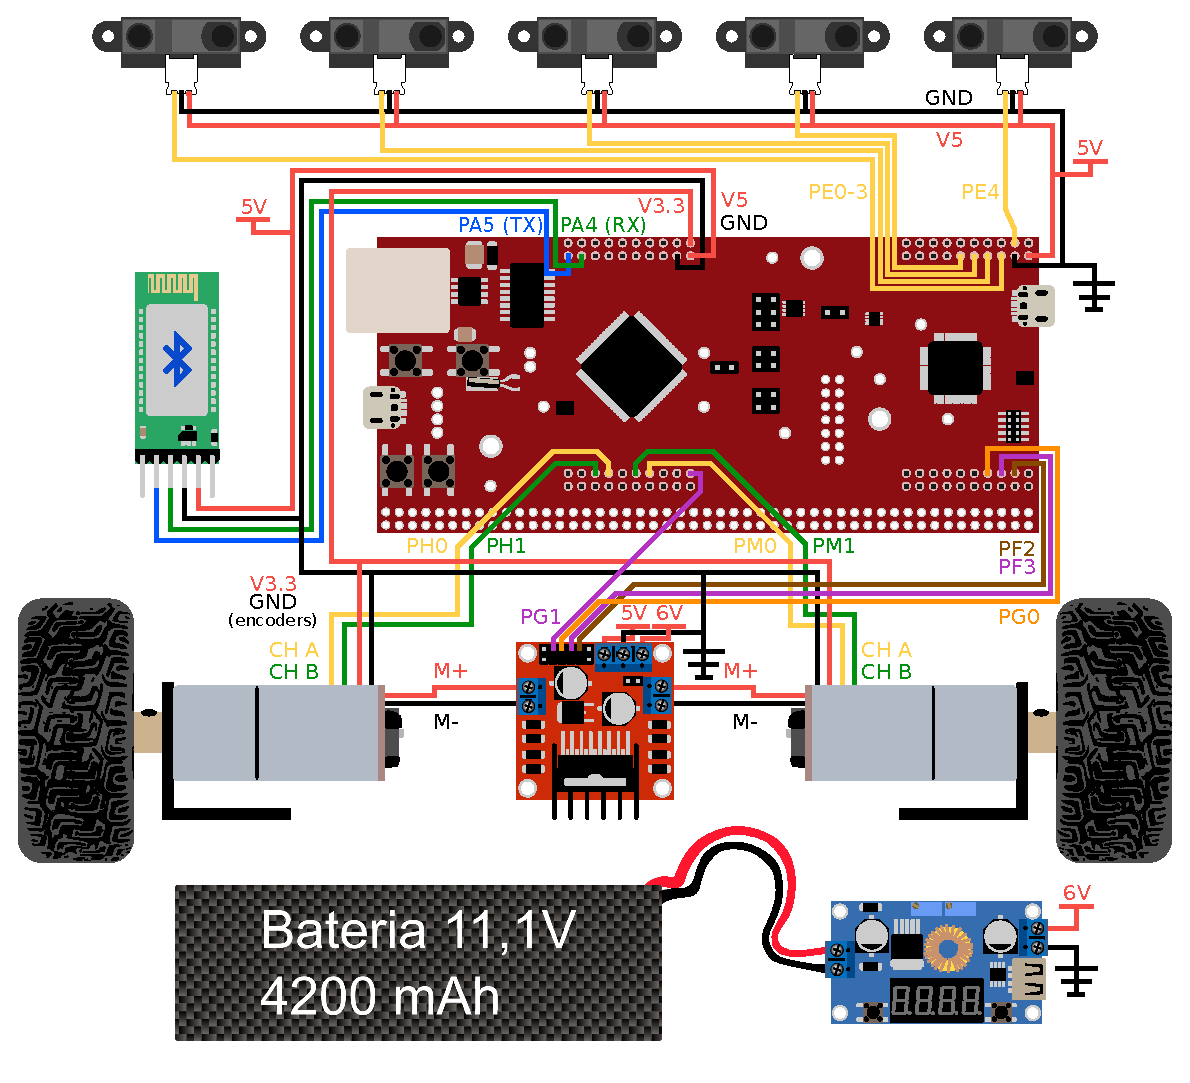
\includegraphics[trim =
		{0cm 0cm 0cm 0cm}, clip, scale=0.8]{Figuras/EsquemaCircuito.eps}};
	\end{tikzpicture}
% 	\vspace{-1cm}
	\label{fig:esquemaCircuito}
	\textbf{Fonte: autoria própria}
\end{figure}
	
	O regulador de tensão foi ajustado para produzir saída de 6 \textit{volts}, pois o 
	acionamento dos motores requer esse nível de tensão. Além dessa saída de 6 \textit{volts}, 
	são necessárias saidas de 3,3 \textit{volts} para microcontrolador e \textit{encoders}, 
	além de saída de 5 \textit{volts} para módulo \textit{bluetooth} e sensores infravermelho. 
	
	Durante fase de projeto, verificou-se que o \textit{driver} ``L298N'' possui internamente 
	um regulador de tensão para obter 5 \textit{volts}. O microcontrolador, por sua vez, tem 
	um regulador interno para obter 3,3 \textit{volts} a partir de 5 \textit{volts} de entrada. 
	
	A escolha de utilizar o regulador interno ao driver parecia uma decisão sagaz, porém
	mostrou-se um fiasco, já que a queda de tensão nele é maior que 1 \textit{volt}. Dessa 
	forma, com a entrada de 6 \textit{volts}, a saída obtida foi menor que os 5 \textit{volts} 
	teoricamente ``prometidos''. Apesar do microcontrolador funcionar, os sensores 
	infravermelho tiveram funcionamento bastante imprevisível, ora medindo adequadamente, 
	ora medindo com erro. 
	
	Uma boa solução para este problema é utilizar outro regulador de tensão para obter 
	5 \textit{volts} a partir da tensão da bateria. Contudo, outra solução foi adotada:
	em vez de utilizar 6 \textit{volts} nos motores, foi utilizado valor de 7 
	\textit{volts}, o que compensa as quedas de tensão do regulador interno ao 
	\textit{driver}. No cálculo de PWM, portanto, deve-se garantir que a tensão média nos 
	motores não ultrapasse os 6 \textit{volts}, para que não funcionem além da 
	especificação. Com essa modificação, foi possível continuar o desenvolvimento e 
	validação dos algoritmos deste trabalho.
	
	\subsection{Configuração de portas no microcontrolador}
	
	O microcontrolador utilizado neste trabalho possui dois módulos
	ADC, com até 20 canais. Cada ADC pode ser usado para a conversão de mais de um canal sem
	intervenção do processador, por meio de um \textit{hardware} chamado sequenciador de 
	amostra (\textit{sample sequencer}). Estas informações podem ser vistas no 
	\textit{datasheet} \cite{datasheet:TivaC}, a partir da página 1053.
	
	As portas ``PE0'' a ``PE4'', conectadas aos sensores IR foram configuradas como entradas
	para conversores AD, de maneira distribuída, com os canais 1 a 3 (portas ``PE2'' a ``PE0'')
	vinculados ao conversor ``ADC0'' e os canais 0 (``PE3'') e 9 (``PE4'') utilizando o 
	conversor ``ADC1''. A associação entre portas e canais podem ser vistos na tabela da 
	página 1055 do \textit{datasheet} \cite{datasheet:TivaC}. 
	
	O microcontrolador usado possui um módulo PWM com quatro blocos de geradores de sinal. 
	Cada gerador de sinal, por sua vez, pode ter sua saída vinculada a duas portas distintas,
	dando um total de oito saídas de PWM. Além disso, existem geradores de banda morta, que 
	são usados para evitar curto-circuitos em uma ``ponte H'' (\textit{driver}). Os 
	curtos-circuitos em uma ``ponte H'' são causados porque seus transistores internos 
	não ``ligam'' e ``desligam'' instantaneamente. Assim, o gerador de banda morta cria 
	dois sinais opostos (o segundo canal é invertido) e com \textit{delays} para a mudança 
	de nível, a fim de ``respeitar'' a dinâmica dos transistores do driver. Estas informações 
	podem ser vistas a patir da página 1669 do \textit{datasheet} \cite{datasheet:TivaC}. A 
	geração de banda morta é explicada brevemente na página 1675.
	
	As portas ``PF2'' e ``PF3" estão associadas às saídas ``PWM2'' e ``PWM3'' (gerador
	1), enquanto as portas portas ``PG0'' e ``PG1'' estão vinculadas às saídas ``PWM4'' e 
	``PWM5'' (gerador 2). A associação entre portas e saídas PWM podem ser vistos na tabela 
	da página 1672 do \textit{datasheet} \cite{datasheet:TivaC}. As portas ``PF'' foram
	conectadas às entradas lógicas do \textit{driver} para o motor esquerdo e as portas 
	``PG'', às entradas do \textit{driver} referentes ao motor direito.

	As portas ``PH0'' e ``PH1'' foram configuradas para \textit{encoders} do motor esquerdo e
	as portas ``PM0'' e ``PM1'' para \textit{encoders} do motor direito. Estas portas foram 
	configuradas como entradas lógicas. Interrupções por borda de descida e subida foram
	configuradas para as portas ``PH0'' e ``PM0'' (canais A dos \textit{encoders} dos motores
	esquerdo e direito, respectivamente). Ao detectar uma interrução em ``PH0'', verificam-se 
	os níveis lógicos das portas ``PH0'' e ``PH1''. A comparação efetuada foi explicada na 
	Seção \ref{SEC:ODOMETRIA}.

	Para comunicação com o módulo \textit{bluetooth} foi utilizada a comunicação ``UART''. O
	microcontrolador utilizado possui oito destes módulos. A ``UART3'' foi configurada
	para as portas ``PA4'' e ``PA5'' (RX e TX, respectivamente). Vale salientar que o receptor
	(RX) do microcontrolador deve se conectar ao transmissor (TX) do módulo \textit{bluetooth} 
	e vice-versa. Portanto, os rótulos RX e TX da Figura \ref{fig:esquemaCircuito} são 
	especificações para o microcontrolador. A associação entre portas e sinais RX e TX do
	módulo ``UART'' podem ser vistos na tabela da página 1163 do \textit{datasheet} 
	\cite{datasheet:TivaC}. 
	
	\subsection{Projeto da placa}
	
	Uma placa foi projetada no intuito de relacionar as portas do microcontrolador
	aos pinos utilizados pelos periféricos e assim, servir de interface. A Figura 
	\ref{fig:JubileuBoard} mostra o circuito projetado com o \textit{software} ``Kicad''. 
	O capacitor indicado na placa possui valor de $1000 \mu F$, que é maior que o necessário.
	
	\begin{figure}[ht]%
	\centering%
	\caption{Placa projetada}%
	\begin{tikzpicture}%
		\node[anchor=south west,inner sep=0] (image) at (0,0) {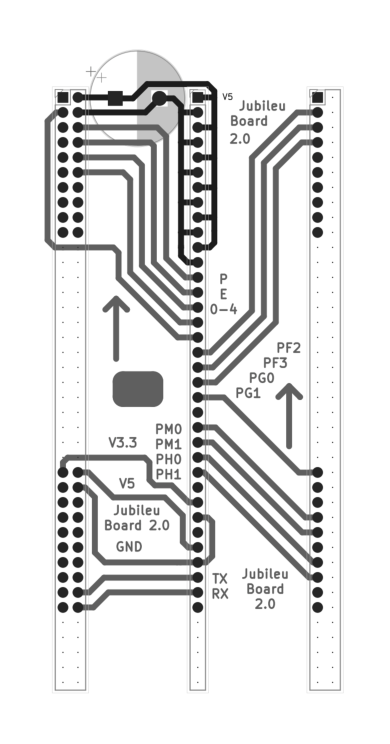
\includegraphics[trim =
		{0cm 0cm 0cm 0cm}, clip,scale=1]{Figuras/JubileuBoard.eps}};%
	\end{tikzpicture}%
	\label{fig:JubileuBoard}%
	
	\textbf{Fonte: autoria própria}%
\end{figure}%
	
	\subsection{Esquema lógico do sistema embarcado}
	
	Em nível de implementação, é uma boa prática de engenharia de \textit{software} definir
	uma arquitetura capaz de abranger os diferentes requisitos. Como este trabalho utiliza 
	dois tipos de controle, híbrido e \textit{fuzzy}, para o código funcionar genericamente, 
	a estratégia de fusão de comportamentos foi transformada em um autômato híbrido com dois 
	estados: ``Parar'' e ``Andar''. ``Parar'' toma controle quando o robô está no objetivo e 
	quando deixa de estar (por alteração da coordenada objetivo) o comportamento ``Andar'' 
	toma conta. Efetivamente, ainda é fusão de comportamentos, pois no estado ``Andar'' todos 
	os comportamentos são calculados e mesclados em uma única recomendação, mas em termos de 
	implementação, utiliza-se uma mesma arquitetura de autômatos.
	
	Portanto, são dois autômatos (supervisores), um para arbitragem e outro para fusão de 
	comportamentos. A fim de selecionar entre estratégias de controle, um autômato com dois
	estados ficou responsável por selecionar o supervisor utilizado. A grosso modo, é um 
	autômato de seleção de supervisores. 
	
	Uma pequena interface por linha de comando via \textit{bluetooth} foi implementada no 
	sistema embarcado e é responsável por definir estratégias de controle que serão utilizadas 
	na navegação, bem como estipular a coordenada objetivo e também para facilitar depuração. 
	O nome desses comandos e respectivas descrições podem ser vistos na Tabela 
	\ref{tab:comunicacaoComandos}. 
	
	\begin{table}[ht]
\centering
\caption{Comandos disponíveis na interface por linha de comando via \textit{bluetooth}}
\vspace{0.2 cm}
\begin{tabular}{|l|l|}
\hline
\textbf{Comando}       & \textbf{Descrição}                                                                                                                     \\ \hline
SUPERVISOR\_HIBRIDO    & \begin{tabular}[c]{@{}l@{}}Adota o controlador híbrido como a estratégia de \\ navegação utilizada\end{tabular}                        \\ \hline
SUPERVISOR\_FUZZY      & \begin{tabular}[c]{@{}l@{}}Adota o controlador \textit{fuzzy} como a estratégia de\\ navegação utilizada\end{tabular}                  \\ \hline
SETCOORDOBJ(X.XX,Y.YY) & Redefine a coordenada objetivo                                                                                                         \\ \hline
GETSTATE               & \begin{tabular}[c]{@{}l@{}}Utilizado para obter a resposta do estado do robô\\ ($x$, $y$ e $\theta$) a cada iteração, bem como o valor de seus\\ sensores \end{tabular}      \\ \hline
EXIT                   & \begin{tabular}[c]{@{}l@{}}Necessário para solicitar ao robô para que deixe \\ de informar seu estado a cada iteração\end{tabular}     \\ \hline
\end{tabular}
\label{tab:comunicacaoComandos}
\end{table}
	
	%\subsection{Implementação da abordagem Híbrida}
	
	%FALTANDO 
	
	%\subsection{Implementação da solução \textit{Fuzzy}}
	
	%FALTANDO
	
\section{Simulação}

	Nesta seção pretende-se mostrar resultados de simulação para as estratégias de 
	arbitragem e fusão de comportamentos. 
	
	O código oficial para o simulador Simiam se encontra no repositório \textit{Github}
	em \citeonline{repositorioSimulacaoOriginal}. O código da simulação deste trabalho 
	é um ``\textit{fork}'' (ramificação de código) do repositório oficial e pode ser 
	consultado em \citeonline{repositorioSimulacaoFork}.
	
	\subsection{Utilizando controlador Híbrido}
	
	A simulação para o controlador híbrido pode ser vista na Figura 
	\ref{fig:resultadoSimulacaoHibrido}. A sequência das 4 imagens pode ser entendida 
	analisando no sentido de leitura: da esquerda para direita, de cima para baixo. O 
	robô adota comportamento ``Ir para Objetivo'' na primeira imagem e, quando encontra 
	o obstáculo em formato côncavo (\textit{frame} 2), adota o comportamento mesclado 
	``Ir para objetivo e Evitar Obstáculos''. Após o \textit{frame} 2, o robô adota o 
	comportamento ``Seguir Parede''. No restante do trajeto, (\textit{frames} 3 e 4) há 
	uma troca constante entre os comportamentos ``Ir para Objetivo'' e ``Mesclado''.
	
	\begin{figure}[ht]
\centering
\caption{Resultado em simulação para o controlador híbrido}
\label{fig:resultadoSimulacaoHibrido}
		\centering
		% fbox{}
		%\includegraphics[clip, 
%scale=0.058]{Figuras/simulacao_hibrido}
		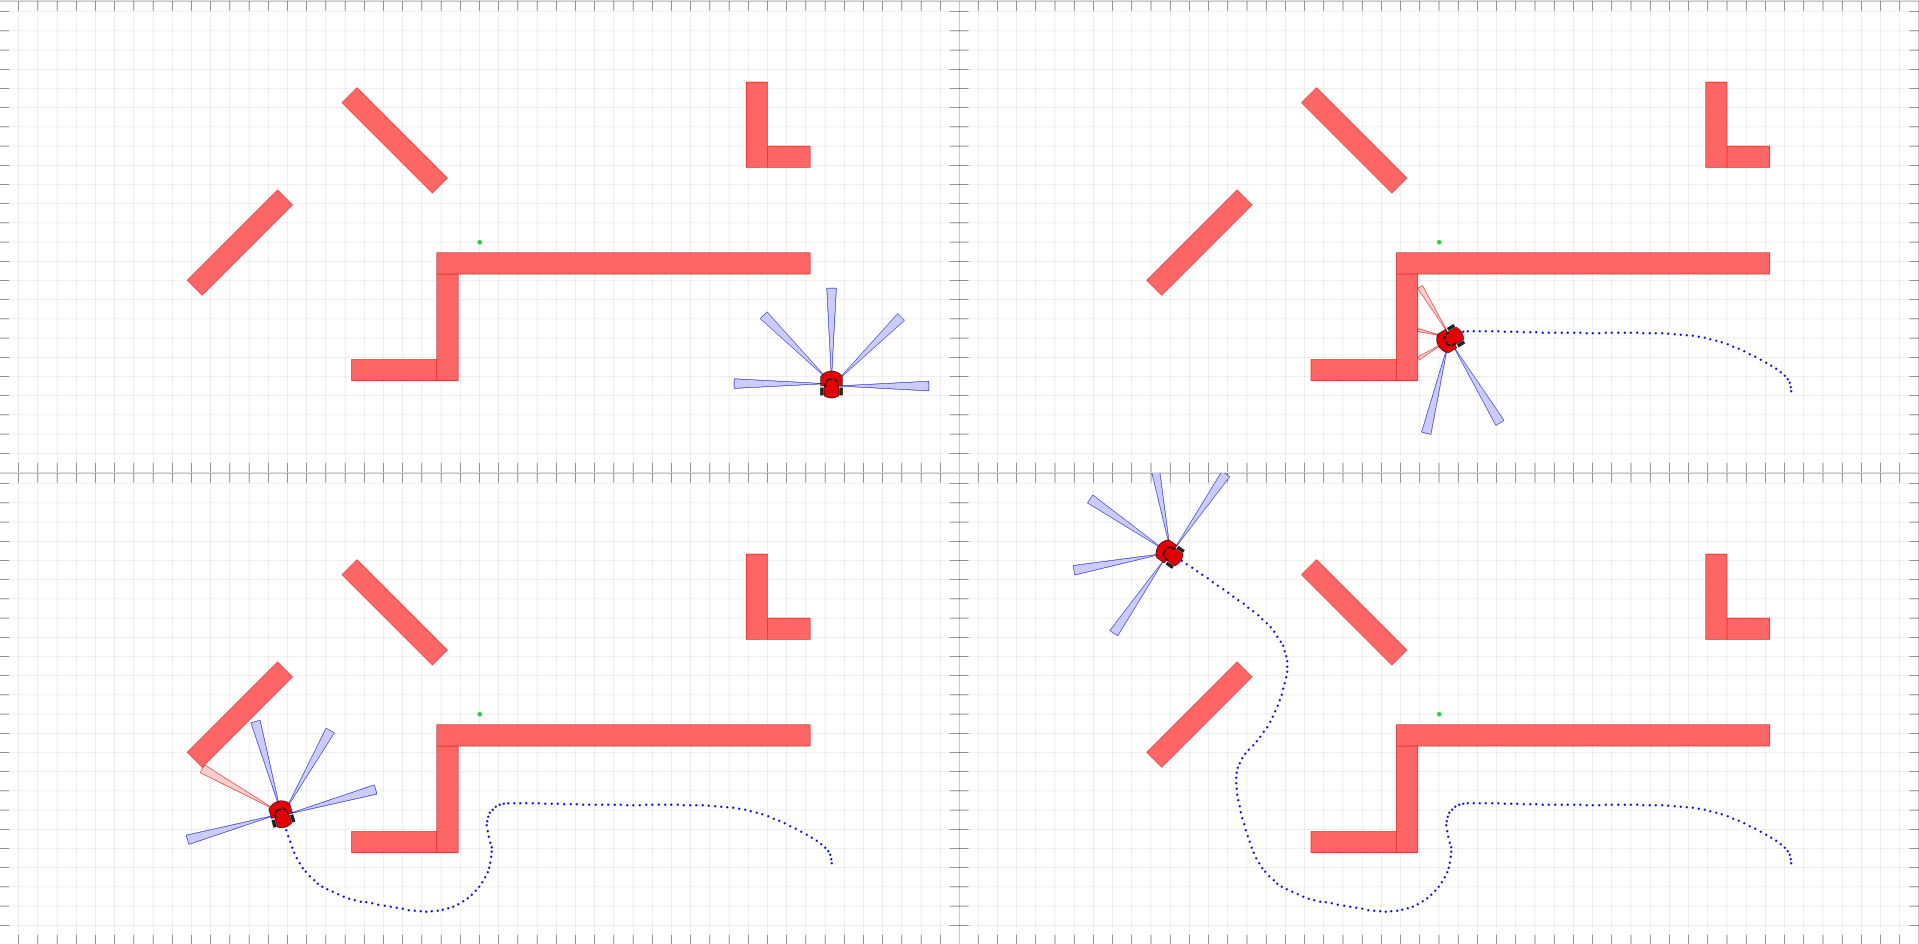
\includegraphics[clip, 
scale=0.232]{Figuras/simulacao_hibrido2Compactado}
		
	\textbf{Fonte: autoria própria}
\end{figure}
	
	A fim de facilitar o entendimento da Figura, o video desta simulação está hospedado
	no Youtube, disponível em \citeonline{youtube:simHibrido}.
	
	O comportamento ``Evitar Obstáculos'' ocorre apenas em situações muito específicas
	(emergenciais), normalmente quando algum obstáculo pequeno está em um ponto cego do 
	robô, ou quando o sentido de movimento forma ângulo de 90 graus com o obstáculo. Em 
	simulação a inércia não é considerada (simulação considera apenas cinemática). Na 
	prática, a inércia é outro motivo para a adoção deste comportamento. O resultado 
	deste comportamento será mostrado no robô real.
	
	\subsection{Utilizando controlador \textit{Fuzzy}}
	
	A simulação para o sistema \textit{Fuzzy} pode ser vista na Figura 
	\ref{fig:resultadoSimulacaoFuzzy}. Aqui, por conta da arquitetura de fusão de 
	comportamentos (com arquitetura de subsunção), existem muitas oscilações, que 
	ocorrem quando o robô precisa decidir entre ``Seguir Parede'' ou ``Ir Para Objetivo''. 
	Como a arquitetura de subsunção é implementada com um contador que determina um peso 
	para combinar linearmente dois comportamentos, oscilações no valor desse contador 
	provocam oscilações na saída. Um pouco antes do segundo \textit{frame}, o robô chega 
	a ficar parado por um tempo até o contador ter um valor suficiente para mudar a 
	recomendação. 
	
	\begin{figure}[ht]
\centering
\caption{Resultado em simulação para o controlador \textit{fuzzy}}
\label{fig:resultadoSimulacaoFuzzy}
		\centering
		% fbox{}
		\includegraphics[clip, 
scale=0.058]{Figuras/simulacao_fuzzy}

	\textbf{Fonte: autoria própria}
\end{figure}
	
	O video desta simulação está hospedado no Youtube, disponível em 
	\citeonline{youtube:simFuzzy}.
	
\section{Resultado e Discussão}

	Nesta seção, pretende-se mostrar resultados de implementação para as estratégias de 
	arbitragem e fusão de comportamentos, além de discutir vantagens e desvantagens destas 
	arquiteturas.
	
	O ambiente utilizado para verificação do resultado é similar ao ambiente de simulação, mas não tem a mesma
	escala, por que a área disponível é menor. Vale salientar que quanto mais se popula o ambiente com obstáculos,
	mais ele se parece com um labirinto. Neste caso, a arquitetura deliberativa seria mais apropriada do que a 
	arquitetura baseada em comportamento. Por isso que o ambiente de testes adotado é um ambiente esparsamente 
	populado.
	
	O código implementado para o microcontrolador pode ser consultado pelo repositório 
	\textit{Github} em \citeonline{repositorioImplementacao}.
	 
	\subsection{Resultado para controlador híbrido}
	
	Nesta subseção, pretende-se mostrar todos os comportamentos separadamente para 
	depois apresentar o resultado com a lógica de arbitragem de comportamentos.
	
	\subsubsection{Comportamento Ir Para Objetivo}
	
	O resultado para o comportamento ``Ir para Objetivo'' pode ser visto na Figura
	\ref{fig:resultadoImplementadoIPO}. O ângulo de referência do robô converge rapidamente
	e, sem obstáculos, o robô segue com agilidade até o objetivo.
	
	\begin{figure}[!ht]
\centering
\caption{Resultado do comportamento ``Ir Para Objetivo''}
\label{fig:resultadoImplementadoIPO}
		\centering
		% fbox{}
		\includegraphics[clip, 
scale=0.058]{Figuras/ComportamentoIPO}%

	\textbf{Fonte: autoria própria}
\end{figure}
	
	A fim de facilitar o entendimento da Figura, o video deste comportamento está 
	hospedado no Youtube, disponível em \citeonline{youtube:IPO}.
	
	\subsubsection{Comportamento Evitar Obstáculo}
	
	O resultado para o comportamento ``Evitar Obstáculo'' pode ser visto na Figura	
	\ref{fig:resultadoImplementadoEO}. O robô sempre busca adotar o caminho contrário
	ao obstáculo percebido, o que explica os movimentos de deflexão observados na Figura.
	
	\begin{figure}[!ht]
\centering
\caption{Resultado do comportamento ``Evitar Obstáculo''}
\label{fig:resultadoImplementadoEO}
		\centering
		% fbox{}
		%\includegraphics[clip, 
%scale=0.058]{Figuras/ComportamentoEO}%
		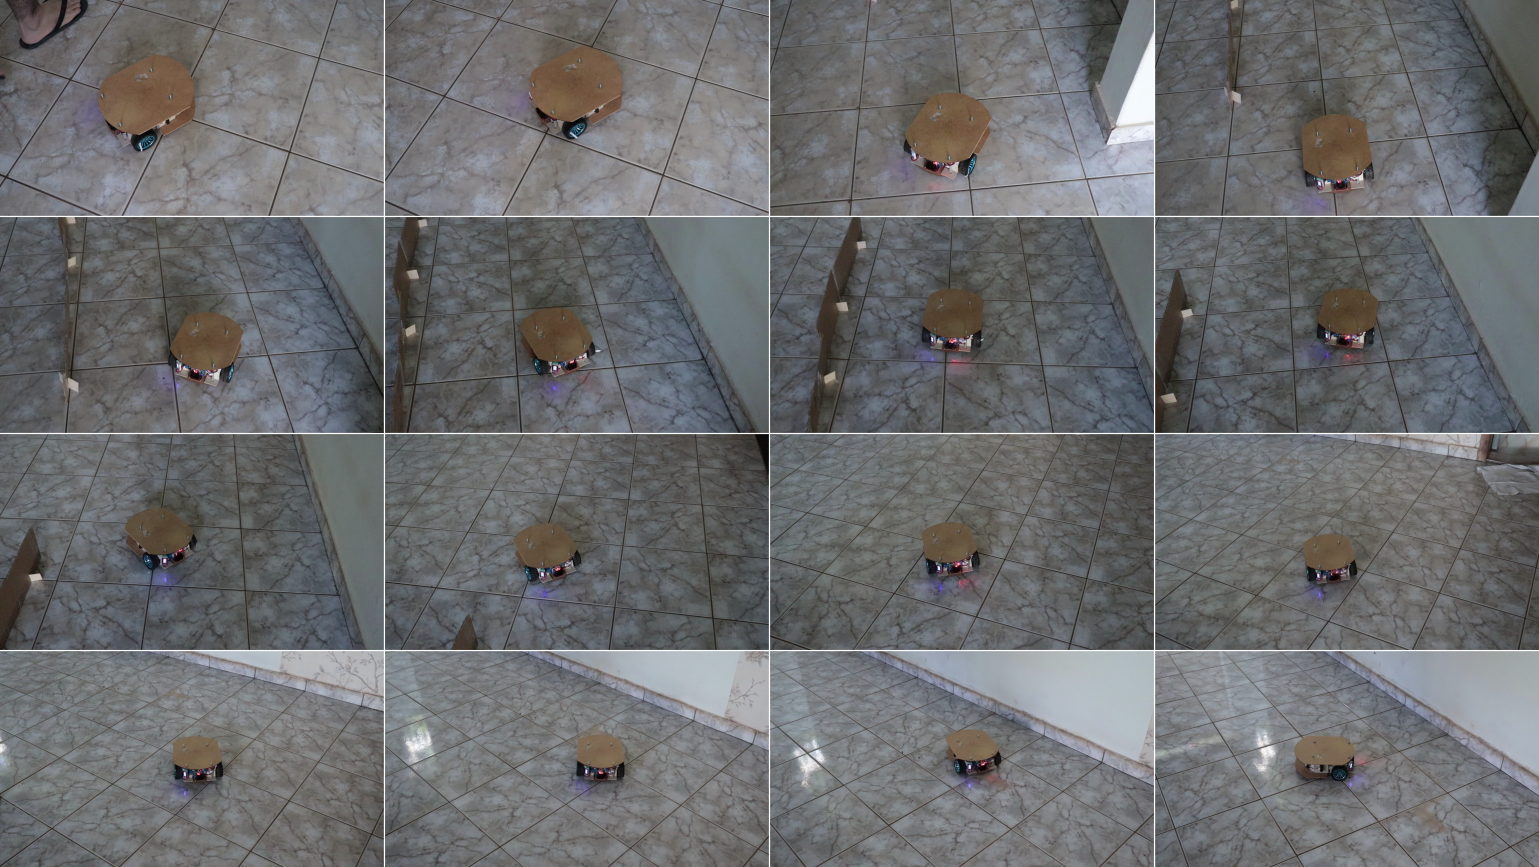
\includegraphics[clip, 
scale=0.29]{Figuras/ComportamentoEOCompactado}%

	\textbf{Fonte: autoria própria}
\end{figure}
	
	A fim de facilitar o entendimento da Figura, o video deste comportamento está 
	hospedado no Youtube, disponível em \citeonline{youtube:EO}.
	
	\subsubsection{Comportamento Mesclado}
	
	O resultado para o comportamento mesclado ``Ir para Objetivo e Evitar Obstáculo'' pode 
	ser visto na Figura \ref{fig:resultadoImplementadoMesclado}. Com este comportamento
	o robô é capaz de navegar em ambientes sem mínimos locais.   
	
	\begin{figure}[!ht]
\centering
\caption{Resultado do comportamento ``Mesclado''}
\label{fig:resultadoImplementadoMesclado}
		\centering
		% fbox{}
		%\includegraphics[clip, 
%scale=0.058]{Figuras/ComportamentoIPO_E_EO}%
		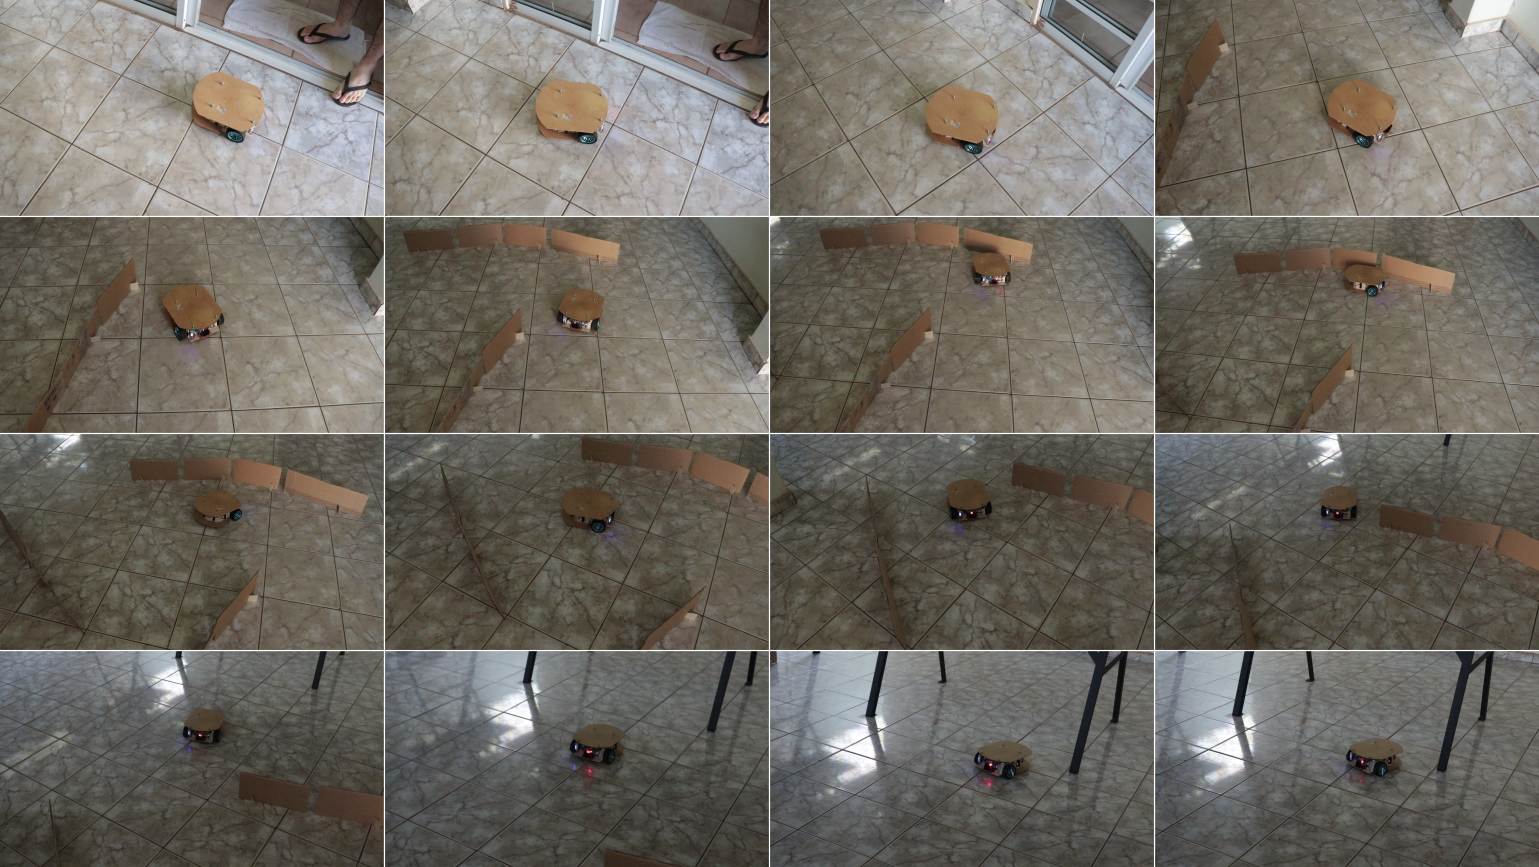
\includegraphics[clip, 
scale=0.29]{Figuras/ComportamentoIPO_E_EOCompactado}%

	\textbf{Fonte: autoria própria}
\end{figure}
	
	A fim de facilitar o entendimento da Figura, o video deste comportamento está 
	hospedado no Youtube, disponível em \citeonline{youtube:IPO_EO}.
	
	\subsubsection{Comportamento Seguir Parede}
	
	O resultado para o comportamento ``Seguir Parede'' pode ser visto na Figura
	\ref{fig:resultadoImplementadoSP}. O sentido horário de contorno foi adotado
	e o robô contorna indefinidamente a parede. É papel do autômato definir o sentido 
	antes de iniciar a execução do controlador.
	
	\begin{figure}[!ht]
\centering
\caption{Resultado do comportamento ``Seguir Parede''}
\label{fig:resultadoImplementadoSP}
		\centering
		% fbox{}
		%\includegraphics[clip, 
%scale=0.058]{Figuras/ComportamentoSP}%
		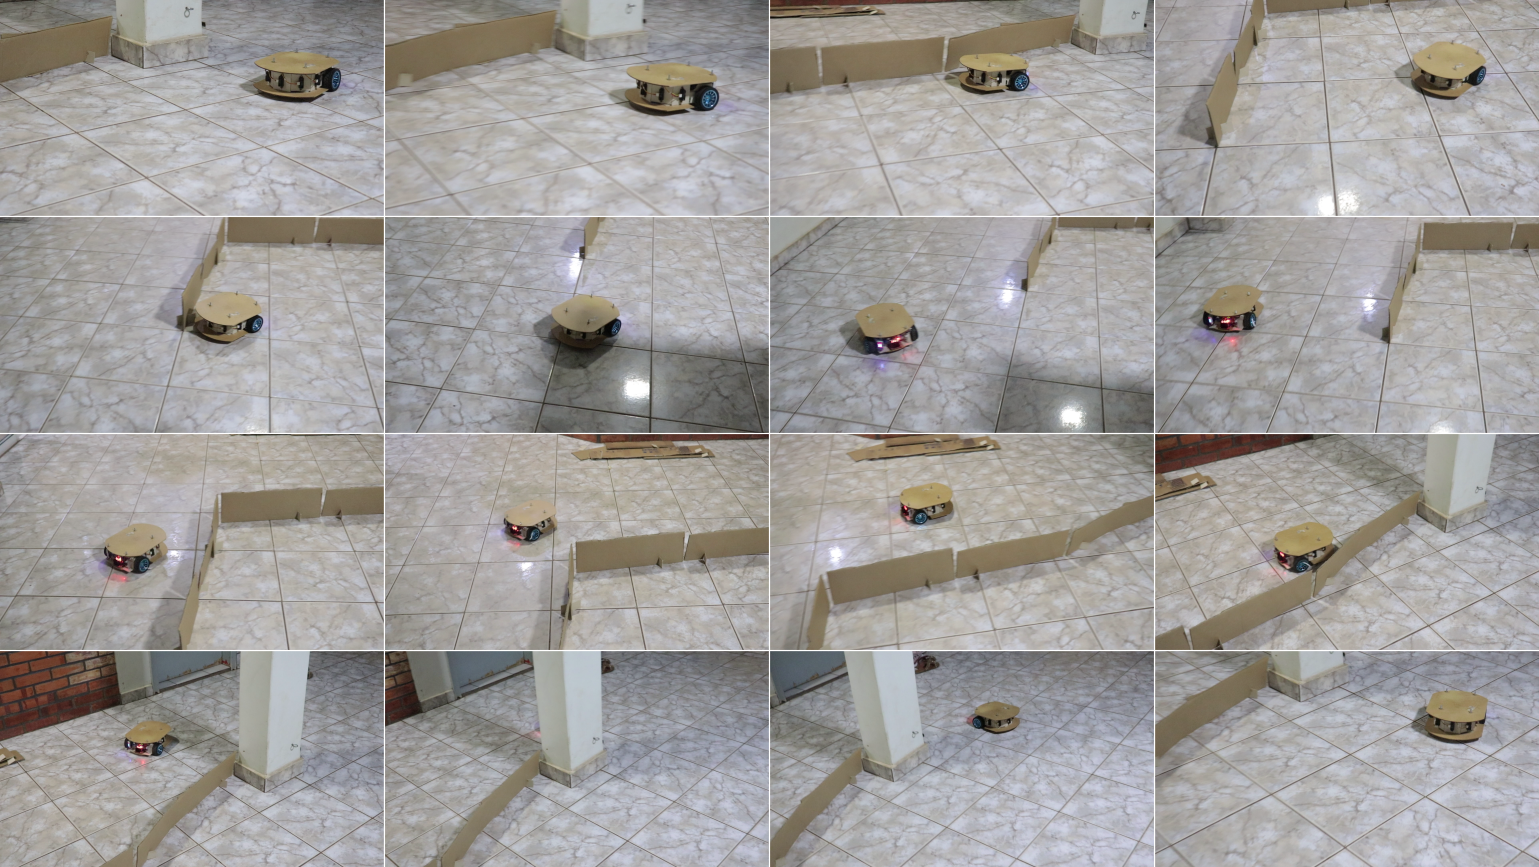
\includegraphics[clip, 
scale=0.29]{Figuras/ComportamentoSPCompactado}%

	\textbf{Fonte: autoria própria}
\end{figure}
	
	A fim de facilitar o entendimento da Figura, o video deste comportamento está 
	hospedado no Youtube, disponível em \citeonline{youtube:SP}.
	
	\subsubsection{Controlador Final com arbitragem}

	A Figura \ref{fig:resultadoImplementadoHibrido} mostra o resultado para o controlador híbrido no robô real.
	A mesma sequência de trocas entre comportamentos acontece aqui, mas por conta de efeitos de inércia e ruído
	nos sensores, ocorrem mudanças mais intensas entre comportamentos do que em simulação.
	
	\begin{figure}[ht]
\centering
\caption{Resultado implementado para o controlador híbrido}
\label{fig:resultadoImplementadoHibrido}
		\centering
		% fbox{}
		%\includegraphics[clip, 
%scale=0.058]{Figuras/hibrido}%
		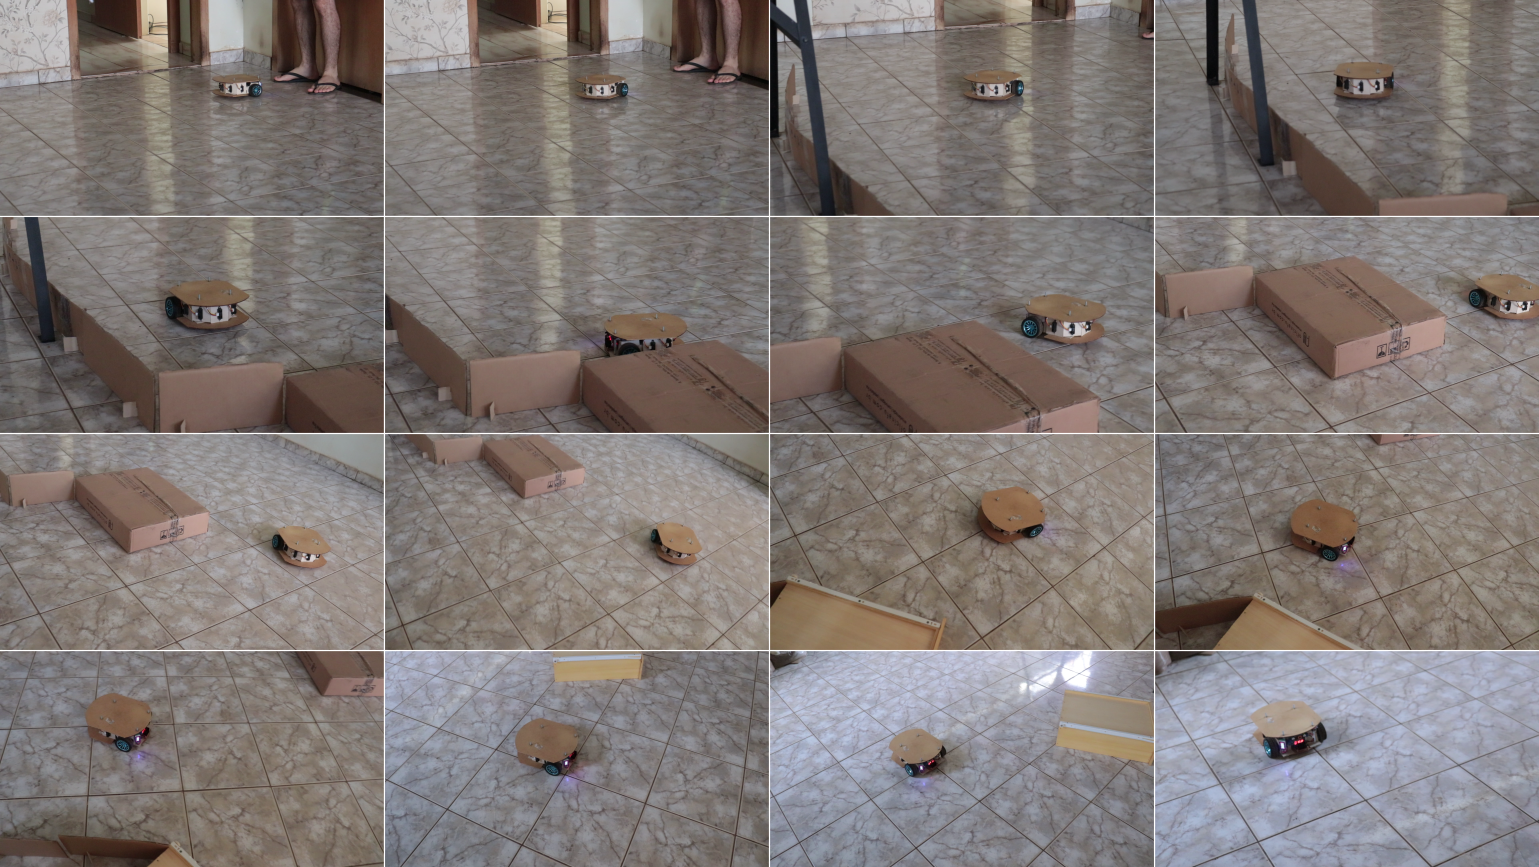
\includegraphics[clip, 
scale=0.29]{Figuras/hibridoCompactado}%

	\textbf{Fonte: autoria própria}
\end{figure}
	
	A fim de facilitar o entendimento da Figura, o video do resultado final para a 
	estratégia de arbitragem de comportamentos está hospedado no Youtube, disponível 
	em \citeonline{youtube:finalHibrido}.
	
	Durante a execução deste trabalho, verificou-se que a arquitetura de arbitragem de comportamentos pode ter 
	um problema muito grave quando há presença de ruído. Nessa situação, o autômato pode fazer uma transição de 
	estado indevida. Quando a transição ocorre para um estado no qual não há transição de retorno para o estado
	anterior, o robô não funciona de acordo com o que foi projetado em simulação e pode ficar preso em mínimos 
	locais ou escolher seguir parede para o lado errado e com isso se chocar com obstáculos.
	
	Nos sensores utilizados neste trabalho, acontece um tipo de ruído que não pôde ser evitado: em questão de 
	poucas iterações (entre 1 e 4) o sensor detecta obstáculo onde não tem. Neste caso, o sensor está detectando
	uma distância de saturação de 80 centímetros quando, de repente, há uma queda para cerca de 40 centímetros, que
	logo volta para o valor anterior. 
	
	O motivo deste ruído não foi descoberto, mas foi ponderado que pode ser alguma queda de tensão no circuito. 
	Por não ter equipamento (osciloscópio) para testar esse palpite, algumas mudanças foram feitas em software. 
	Foi implementado um filtro de média móvel com janela de 5 iterações para reduzir o efeito do ruído. Mas este
	valor filtrado foi utilizado apenas para verificar se é necessário fazer transições de estado. Para executar
	os controladores, utilizou-se o valor real com ruído mesmo. Isso foge um pouco da arquitetura baseada em 
	comportamento, já que os componentes dessa arquitetura precisam ser reativos (valores atuais, sem considerar 
	o passado do sistema). Deste modo, os comportamentos são reativos, mas o processo de ``decisão'' 
	não pode ser classificado como tal, pois utiliza estados anteriores do sistema.
	
	Além dessa alteração, foi definida uma saturação para os sensores diagonais e frontais. Quando estes sensores
	detectam valores maiores do que 70 centímetros, estes valores são alterados para 80 centímetros, a fim de
	reduzir o efeito dos ruídos no comportamento.  
	
	\subsection{Resultado para controlador \textit{fuzzy}}

	A Figura \ref{fig:resultadoImplementadoFuzzy} mostra o resultado para o controlador \textit{Fuzzy} no robô 
	real. Aqui, por conta de ruído, o robô não chega a parar quando está prestes a adotar o comportamento de 
	``Seguir Parede''. Ele oscila na região de mínimo local, o que pode ser constatado verificando os 
	\textit{frames} 4 a 8. Nos \textit{frames} 14 a 16, nota-se uma certa lentidão no momento de se aproximar do
	objetivo, pois ocorre uma oscilação entre comportamentos de ``Ir para Objetivo'' e ``Seguir Parede''. Isso 
	pode ser explicado da seguinte forma: a proximidade do objetivo leva a uma recomendação de velocidade pequena e
	o atrito dos motores faz o robô parar. Deixando de fazer progresso, o contador da arquitetura de subsunção 
	aumenta o peso para o comportamento de ``Seguir Parede'', o que faz o robô voltar a fazer progresso e o 
	valor do contador diminui novamente. Por isso o robô para e anda de pouco a pouco até chegar no objetivo.
	
	\begin{figure}[ht]
\centering
\caption{Resultado implementado para o controlador \textit{fuzzy}}
\label{fig:resultadoImplementadoFuzzy}
		\centering
		% fbox{}
		%\includegraphics[clip, 
%scale=0.058]{Figuras/fuzzy}
		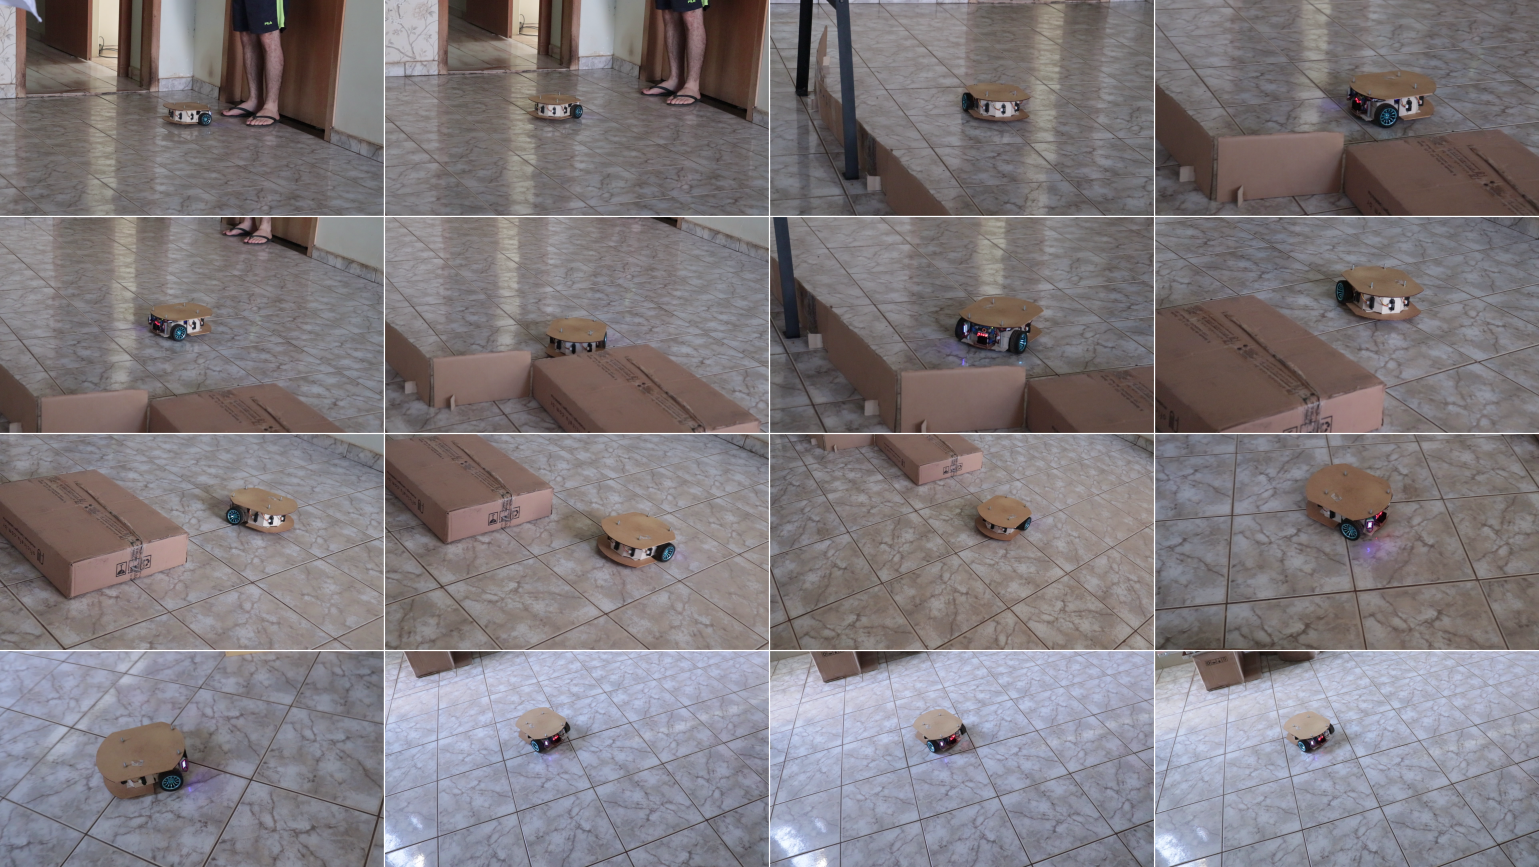
\includegraphics[clip, 
scale=0.29]{Figuras/fuzzyCompactado}

	\textbf{Fonte: autoria própria}
\end{figure}

	A fim de facilitar o entendimento da Figura, o video do resultado final para a 
	estratégia de fusão de comportamentos está hospedado no Youtube, disponível em 
	\citeonline{youtube:finalFuzzy}.
		
	As oscilações excessivas para o controlador \textit{Fuzzy} são provocadas pela arquitetura de fusão de 
	comportamentos e não pelo sistema \textit{fuzzy} em si.
	
	Os ruídos relatados para a arquitetura de arbitragem de comportamentos também ocorrem aqui. Contudo, apenas 
	a definição de uma saturação para sensores diagonais e central (para valores acima de 70 centímetros) foi 
	suficiente para fazer o controlador funcionar, não sendo necessário nenhum filtro de média móvel. Componentes 
	reativos são muito robustos para sistemas que apresentam ruídos de pouca duração, já que um comportamento 
	errático durará apenas enquanto os ruídos estiverem presentes e, logo a seguir, o controlador retorna ao 
	funcionamento normal.
	
%\chapter{Considerações Finais}
\vspace{-2.5 cm}

Para concluir esta etapa do trabalho, algumas deliberações precisam ser feitas.
Por enquanto, uma parte do trabalho foi completamente desconsiderada: estimativa
do estado do sistema. Para simulação, muitos trabalhos acadêmicos consideram o
estado atual do robô como um valor conhecido. Para um robô real, autônomo, este
estado pode ser estimado usando técnicas como observadores, filtro de Kalman,
odometria, entre outras.

É importante salientar que há um conflito entre os objetivos deste trabalho,
já que um robô ao mesmo tempo autônomo e sem armazenamento de mapa deve possuir
a capacidade de estimar com perfeição seu estado atual. Na prática, a estimativa
de estado carrega erros que são somados no decorrer do tempo de execução. Para
corrigir tais erros, ou o robô deve armazenar mapa (representação interna do
mundo à sua volta) e reconhecer locais já visitados, ou o robô precisa de um
sistema externo (computador com câmera, sistema GPS) que envie correções
(isso reduz autonomia). 

A segunda solução pode ser adotada neste trabalho, a fim de torná-lo mais focado
no aspecto de controle e navegação, o que possibilitará explorar as diferentes
abordagens estipuladas (controle híbrido e \textit{fuzzy}) com maior
aproveitamento. 

Desta forma, uma comparação qualitativa será efetuada. Esta análise
deve ser qualitativa pois não existe um padrão de teste (\textit{benchmark})
amplamente adotado em robótica móvel. Logo, qualquer análise comparativa só pode
ser qualitativa.
\chapter{Conclusões e Trabalhos Futuros}
\vspace{-2.5 cm}

Este trabalho teve por intuito defender que a definição de uma boa arquitetura para solução de um problema é
mais importante que a tecnologia empregada. Com a definição de uma arquitetura robusta, o funcionamento do sistema 
independe de tecnologia. Neste trabalho, por exemplo, utilizou-se controladores PID e controladores \textit{Fuzzy}
para implementar as estratégias de arbitragem e fusão, mas elas poderiam ter sido utilizadas em conjunto sob uma mesma
estratégia. Se um novo comportamento precisar ser implementado, qualquer tecnologia poderia ser usada para 
implementá-lo (desde soluções reativas simples até algoritmos de aprendizado de máquina), o que torna a solução
deste trabalho escalável.

Nesse sentido, é necessário comparar arquiteturas de arbitragem e fusão de comportamento. A primeira é mais escalável
que a segunda, já que cada comportamento pode ser testado de modo isolado. Na fusão de comportamentos, cada novo
comportamento adicionado se relaciona com todos os outros e a complexidade tende a aumentar de maneira exponencial.
O grande problema detectado na arquitetura de arbitragem é a situação de presença de ruído, que foi discutida na seção
dos resultados. Este trabalho adotou uma solução que provavelmente não é a melhor. Filtrar o ruído atrasa a 
``velocidade de percepção'', já que demora mais tempo para que o robô perceba que houve uma mudança no ambiente. 

Talvez exista alguma forma de detectar que o ruído ocorreu e desfazer transições indevidas. É interessante 
investigar em trabalhos futuros uma forma de tornar um autômato mais robusto na presença de ruídos. 

A arquitetura de fusão de comportamentos tem a tendência de provocar muitas oscilações, pois ao integrar 
um novo comportamento, este deve interagir com todos os outros. Em certas circunstâncias ele pode ser suprimido, em
outras, deve ``cancelar'' os outros a fim de se sobressair. As oscilações ocorrem por conta da interação entre 
comportamentos, quando está ora suprimido, ora se sobressaindo em relação aos demais.

A questão do custo computacional é outro ponto onde a arbitragem de comportamentos se sobressai,
pois apenas um comportamento é executado por vez. Desde que cada comportamento execute dentro
do tempo disponível, o custo computacional não compromete o funcionamento. Na fusão de 
comportamentos, por outro lado, todos os custos individuais se somam. 

Outro aspecto importante neste trabalho é a conversão de modelos de acionamento diferencial para uniciclo. Pode 
parecer completamente desnecessário em uma primeira leitura, porém, se houver a necessidade de controlar algum outro 
robô, com outro modelo matemático, em um mesmo ambiente, percebe-se que, desde que seja possível converter seu modelo 
para o uniciclo, o mesmo controlador deste trabalho poderá ser usado para controlá-lo.  
 
Considerando que outros robôs podem se beneficiar do mesmo algoritmo de controle deste trabalho, desde que 
seu modelo possa ser convertido para o uniciclo, seria interessante explorar essa integração em trabalhos futuros.
o robô tipo ``Segway'' seria um bom ponto de partida, já que é necessário apenas um controlador a mais para controlar
o ângulo vertical (controle de um pêndulo invertido), bem como uma forma de associar a inclinação do ``pêndulo'' com 
a velocidade linear do uniciclo.

O presente trabalho teve objetivos muito extensos e, portanto, deixou muitos pontos que são passíveis de melhoria.
Para trabalhos futuros, é interessante investigar melhorias no simulador. Acredito que seria interessante reescrevê-lo
em um ``ambiente'' de código aberto. O ``Gazebo'' do \textit{Robot Operating System} (ROS) pode ser uma boa 
alternativa. Ou talvez, escrever uma espécie de extensão para o Blender, já que o aspecto de renderização já está
implementado e seria possível obter animações muito bonitas ao concluir uma simulação.  

Acredito que melhorias futuras devem levar em conta a importância de definir uma espécie de 
``infraestrutura'' ou ``ecossistema'' para robótica, que seriam ferramentas e sistemas cujas
funcionalidades facilitem o desenvolvimento e testes de robôs. A chave para isso acredito que 
está em desenvolver um simulador mais robusto, capaz de se conectar aos robôs, usar seus
sensores como entrada para o algoritmo a ser testado e devolver o resultado a eles, para que
realizem a atuação recomendada (a Universidade Georgia Tech possui algo nesse sentido para 
os seus robôs Khepera). 

Com essa infraestrutura, é possível testar muito rapidamente quaisquer alterações no algoritmo.
Com a utilização de câmeras, a coordenada do robô real pode ser estimada, de modo a
calcular com maior precisão os erros de odometria, além de facilitar a extração de figuras e
videos para análise posterior. A partir desse ``ecossistema'', um tema mais moderno em robótica 
móvel pode ser explorado: navegação em grupos. 

%Para finalizar, gostaria de salientar que os trabalhos atuais em robótica móvel tratam de 
%temas como navegação em grupo. 

%Essa infraestrutura requer a convergência entre as áreas de Engenharia de 
%Software, Processamento de Imagens e Desenvolvimento Web.
 
%Para finalizar, gostaria de salientar que os trabalhos atuais em robótica móvel tratam de temas como navegação em 
%grupo. Dito isso, para o meu descontentamento, o presente trabalho apenas faz algo que já se fazia na década de 90. 
%As universidades que fazem o que há de mais avançado possuem uma cultura de dar continuidade a trabalhos 
%anteriores. 

%Para isso ser possível na UTFPR, é necessário desenvolver uma espécie de ``infraestrutura'' para robótica. Desenvolver
%ao longo de multiplos trabalhos acadêmicos um conjunto de ferramentas cujas funcionalidades permitiriam integrar 
%simuladores aos robôs reais. Como exemplo, posso imaginar simuladores que permitem exportar código direto para os 
%robôs . Nesse ``ecossistema'' de 
%robótica, sistemas com câmeras poderiam ajudar a desenhar o trajeto do robô e facilitar o processo de depuração.

%Para iniciar a implementação desse grande projeto, é necessário compreender o que são arquiteturas escaláveis para 
%sistemas IOT (internet das coisas). É cada vez mais comum no mundo do software falar de arquitetura 
%de microserviços, mas não está muito claro para o estudante de engenharia de computação como seria a integração das 
%tecnologias de software com dispositivos IOT. É necessário compreender a diferença entre os servidores de 
%mensageria (\textit{brokers}) que são implementados para comunicação entre microserviços e para comunicação entre 
%dispositivos IOT. Eles não são intercambiáveis (pelo menos hoje em dia).  

%É importante falar disso, pois desenvolver um ``ecossistema'' escalável para robótica traria diversas vantagens, já
%que seria mais fácil efetuar testes em robõs e facilitaria a integração de um número maior de robôs operando em um 
%mesmo ambiente. O conhecimento em nível de arquitetura contribui para formar profissionais melhores, tendo em vista 
%que o objetivo do curso de Engenharia de Computação é justamente formar profissionais capazes de integrar 
%\textit{hardware} e \textit{software}.
